% Ciencia Abierta presentation by Washington L. de Carvalho Segundo.
% Licensed under CC BY-NC-SA 4.0.
% https://creativecommons.org/licenses/by-nc-sa/4.0/
\documentclass[aspectratio=169,11pt]{beamer}

\usepackage[T1]{fontenc}
\usepackage[utf8]{inputenc}
\usepackage{lmodern}
\usepackage{fontspec}
\usepackage{graphicx}
\usepackage{tikz}
\usetikzlibrary{positioning,calc}
\usepackage{booktabs}
\usepackage{array}
\usepackage{ragged2e}
\usepackage{hyperref}

% Embedded open fonts ensure that non-Latin scripts compile identically in
% Tectonic and Overleaf. See assets/fonts/OFL.txt for the font license.
\newfontfamily\worldlatin[Path=assets/fonts/]{NotoSans.ttf}
\newfontfamily\devanagarifont[Path=assets/fonts/]{NotoSansDevanagari.ttf}
\newfontfamily\bengalifont[Path=assets/fonts/]{NotoSansBengali.ttf}
\newfontfamily\tamilfont[Path=assets/fonts/]{NotoSansTamil.ttf}
\newfontfamily\ethiopicfont[Path=assets/fonts/]{NotoSansEthiopic.ttf}
\newfontfamily\chinesefont[Path=assets/fonts/]{NotoSansSC.ttf}

\definecolor{Navy}{HTML}{092B4C}
\definecolor{Teal}{HTML}{2B9C9A}
\definecolor{Cyan}{HTML}{54C7D5}
\definecolor{Coral}{HTML}{F47C61}
\definecolor{Mist}{HTML}{EDF6F5}
\definecolor{Warm}{HTML}{FAF7F0}
\definecolor{Ink}{HTML}{163247}
\definecolor{Muted}{HTML}{5C7180}

\setbeamercolor{normal text}{fg=Ink,bg=Warm}
\setbeamercolor{frametitle}{fg=Navy,bg=Warm}
\setbeamercolor{structure}{fg=Teal}
\setbeamercolor{alerted text}{fg=Coral}
\setbeamerfont{frametitle}{series=\bfseries,size=\Large}
\setbeamerfont{title}{series=\bfseries,size=\Huge}
\setbeamerfont{subtitle}{size=\Large}
\setbeamertemplate{navigation symbols}{}
\setbeamertemplate{itemize item}{\color{Coral}\small\raise0.15ex\hbox{$\bullet$}}
\setbeamertemplate{itemize subitem}{\color{Teal}\scriptsize\raise0.15ex\hbox{$\bullet$}}
\setbeamersize{text margin left=0.65cm,text margin right=0.65cm}

\setbeamertemplate{frametitle}{%
  \vspace{0.22cm}\insertframetitle\par
  \vspace{-0.16cm}{\color{Cyan}\rule{1.2cm}{1.6pt}}\vspace{0.1cm}}

\setbeamertemplate{footline}{%
  \leavevmode\hbox{%
  \begin{beamercolorbox}[wd=.88\paperwidth,ht=2.5ex,dp=1.1ex,leftskip=.65cm]{normal text}%
    %\scriptsize\color{Muted}High-Level Conference on International Ciencia Abierta Cooperation, Shanghai, 11 September 2026
  \end{beamercolorbox}%
  \begin{beamercolorbox}[wd=.12\paperwidth,ht=2.5ex,dp=1.1ex,center]{normal text}%
    \scriptsize\color{Muted}\insertframenumber
  \end{beamercolorbox}}}

\newcommand{\tagline}[1]{\textcolor{Teal}{\bfseries\small#1}}
\newcommand{\keypoint}[2]{%
  \begin{minipage}[t]{0.98\linewidth}
  \colorbox{Mist}{\parbox{0.92\linewidth}{\raggedright\vspace{0.08cm}\textcolor{Navy}{\bfseries #1}\par\small #2\vspace{0.08cm}}}
  \end{minipage}}
\newcommand{\stage}[2]{%
  \begin{minipage}[t]{0.18\linewidth}\centering
  \tikz\node[circle,fill=Teal,text=white,minimum size=0.72cm,font=\bfseries] {#1};\\[0.12cm]
  \small\textbf{#2}
  \end{minipage}}

\newcommand{\ccLicenseURL}{https://creativecommons.org/licenses/by-nc-sa/4.0/deed.es}
\newcommand{\serviceqr}[2]{%
  \begin{tikzpicture}[remember picture,overlay]
    \node[anchor=south east,fill=Warm,inner sep=3pt] at
      ([xshift=-.30cm,yshift=.72cm]current page.south east)
      {\href{#1}{\includegraphics[height=1.45cm]{#2}}};
  \end{tikzpicture}}

% The complete license mark appears only on the title and closing slides.
\setbeamertemplate{background}{}

% ---------------------------------------------------------------------------
% Editable monochrome diagrams
% Change labels, positions, and connections directly in the TikZ code below.
\tikzset{
  diagram node/.style={draw=Navy,very thick,fill=Mist,rounded corners=5pt,
    align=center,minimum height=.88cm,text width=2.1cm,font=\small\bfseries,
    text=Navy,inner sep=5pt},
  diagram small/.style={draw=Navy,thick,fill=Mist,rounded corners=4pt,
    align=center,minimum height=.74cm,text width=1.75cm,font=\scriptsize,
    text=Navy,inner sep=4pt},
  diagram arrow/.style={->,>=stealth,very thick,draw=Teal},
  diagram line/.style={thick,draw=Coral}
}

\newcommand{\OpenScienceCycleDiagram}{%
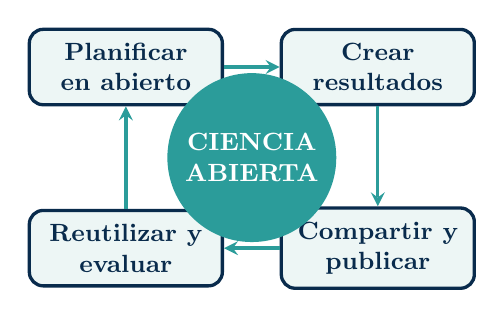
\begin{tikzpicture}
  \node[diagram node] (plan) at (0,1.15) {Planificar\\en abierto};
  \node[diagram node] (create) at (3.2,1.15) {Crear\\resultados};
  \node[diagram node] (share) at (3.2,-1.15) {Compartir y\\publicar};
  \node[diagram node] (reuse) at (0,-1.15) {Reutilizar y\\evaluar};
  \draw[diagram arrow] (plan) -- (create);
  \draw[diagram arrow] (create) -- (share);
  \draw[diagram arrow] (share) -- (reuse);
  \draw[diagram arrow] (reuse) -- (plan);
  \node[draw=Teal,very thick,circle,fill=Teal,align=center,
    font=\bfseries\small,text=white,minimum size=1.20cm] at (1.6,0) {CIENCIA\\ABIERTA};
\end{tikzpicture}}

\newcommand{\KnowledgeValueChainDiagram}{%

\begin{tikzpicture}[node distance=.55cm]
  \node[diagram node] (objects) {Objetos de\\investigación};
  \node[diagram node,right=of objects] (curation) {Curación y\\metadatos};
  \node[diagram node,right=of curation] (analysis) {Análisis y\\modelos};
  \node[diagram node,right=of analysis] (ai) {IA\\responsable};
  \node[diagram node,right=of ai] (value) {Valor\\público};
  \draw[diagram arrow] (objects) -- (curation);
  \draw[diagram arrow] (curation) -- (analysis);
  \draw[diagram arrow] (analysis) -- (ai);
  \draw[diagram arrow] (ai) -- (value);
  \node[font=\scriptsize,text=Muted,align=center,text width=2.1cm,below=.22cm of objects] {Datos y código\\Publicaciones};
  \node[font=\scriptsize,text=Muted,align=center,text width=2.1cm,below=.22cm of curation] {Contexto y\\procedencia};
  \node[font=\scriptsize,text=Muted,align=center,text width=2.1cm,below=.22cm of analysis] {Patrones y\\evidencia};
  \node[font=\scriptsize,text=Muted,align=center,text width=2.1cm,below=.22cm of ai] {Automatización fundamentada};
  \node[font=\scriptsize,text=Muted,align=center,text width=2.1cm,below=.22cm of value] {Decisiones y\\servicios};
\end{tikzpicture}}

\newcommand{\OpenInfrastructureDiagram}{%
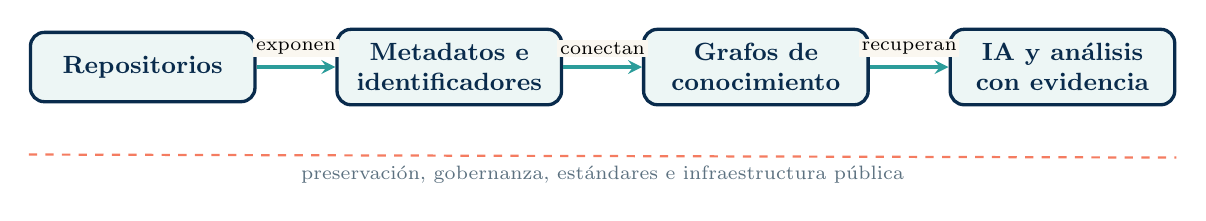
\begin{tikzpicture}[node distance=1.0cm,diagram node/.append style={text width=2.5cm}]
  \node[diagram node] (repo) {Repositorios};
  \node[diagram node,right=of repo] (meta) {Metadatos e\\identificadores};
  \node[diagram node,right=of meta] (graph) {Grafos de\\conocimiento};
  \node[diagram node,right=of graph] (ai) {IA y análisis\\con evidencia};
  \draw[diagram arrow] (repo) -- node[midway,above=3pt,font=\scriptsize,fill=Warm,inner sep=1pt]{exponen} (meta);
  \draw[diagram arrow] (meta) -- node[midway,above=3pt,font=\scriptsize,fill=Warm,inner sep=1pt]{conectan} (graph);
  \draw[diagram arrow] (graph) -- node[midway,above=3pt,font=\scriptsize,fill=Warm,inner sep=1pt]{recuperan} (ai);
  \draw[diagram line,dashed] ([yshift=-.65cm]repo.south west) --
    node[below,font=\scriptsize,text=Muted]{preservación, gobernanza, estándares e infraestructura pública}
    ([yshift=-.65cm]ai.south east);
\end{tikzpicture}}

\newcommand{\BrazilEcosystemDiagram}{%
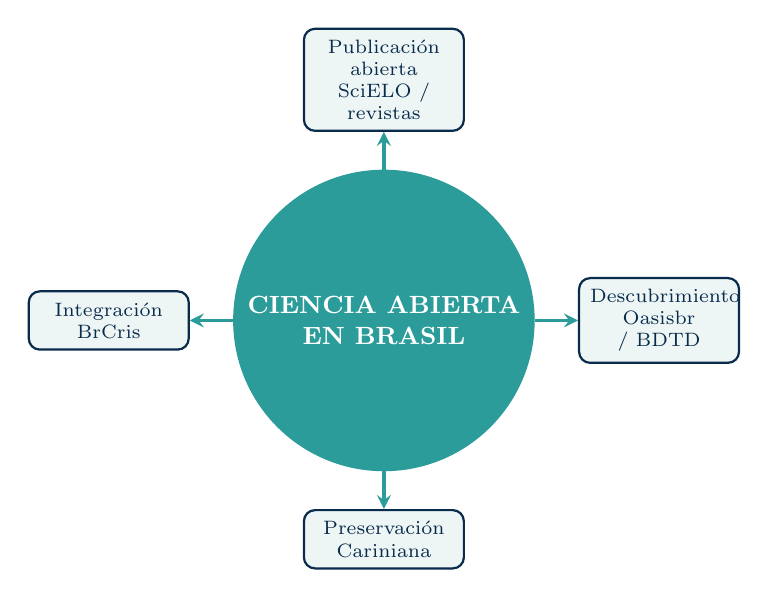
\begin{tikzpicture}[node distance=.48cm and .55cm]
  \node[draw=Teal,very thick,circle,fill=Teal,align=center,
    font=\bfseries\small,text=white,minimum size=1.45cm] (core) {CIENCIA ABIERTA\\EN BRASIL};
  \node[diagram small,above=of core] (publish) {Publicación abierta\\SciELO / revistas};
  \node[diagram small,right=of core] (discover) {Descubrimiento\\Oasisbr / BDTD};
  \node[diagram small,below=of core] (preserve) {Preservación\\Cariniana};
  \node[diagram small,left=of core] (integrate) {Integración\\BrCris};
  \draw[diagram arrow] (core) -- (publish);
  \draw[diagram arrow] (core) -- (discover);
  \draw[diagram arrow] (core) -- (preserve);
  \draw[diagram arrow] (core) -- (integrate);
\end{tikzpicture}}

\newcommand{\SustainableDevelopmentDiagram}{%
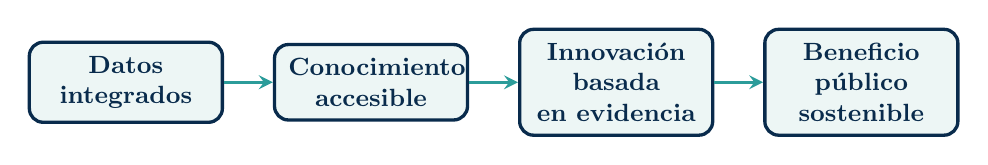
\begin{tikzpicture}[node distance=.62cm]
  \node[diagram node] (data) {Datos\\integrados};
  \node[diagram node,right=of data] (knowledge) {Conocimiento\\accesible};
  \node[diagram node,right=of knowledge] (innovation) {Innovación basada\\en evidencia};
  \node[diagram node,right=of innovation] (benefit) {Beneficio público\\sostenible};
  \draw[diagram arrow] (data) -- (knowledge);
  \draw[diagram arrow] (knowledge) -- (innovation);
  \draw[diagram arrow] (innovation) -- (benefit);
\end{tikzpicture}}

\begin{document}

{\setbeamertemplate{footline}{}\setbeamertemplate{background}{}
% Slide 1
\begin{frame}[plain]
  \begin{tikzpicture}[remember picture,overlay]
    % Background image intentionally disabled.
    % \node[anchor=center,opacity=.30] at (current page.center)
    %   {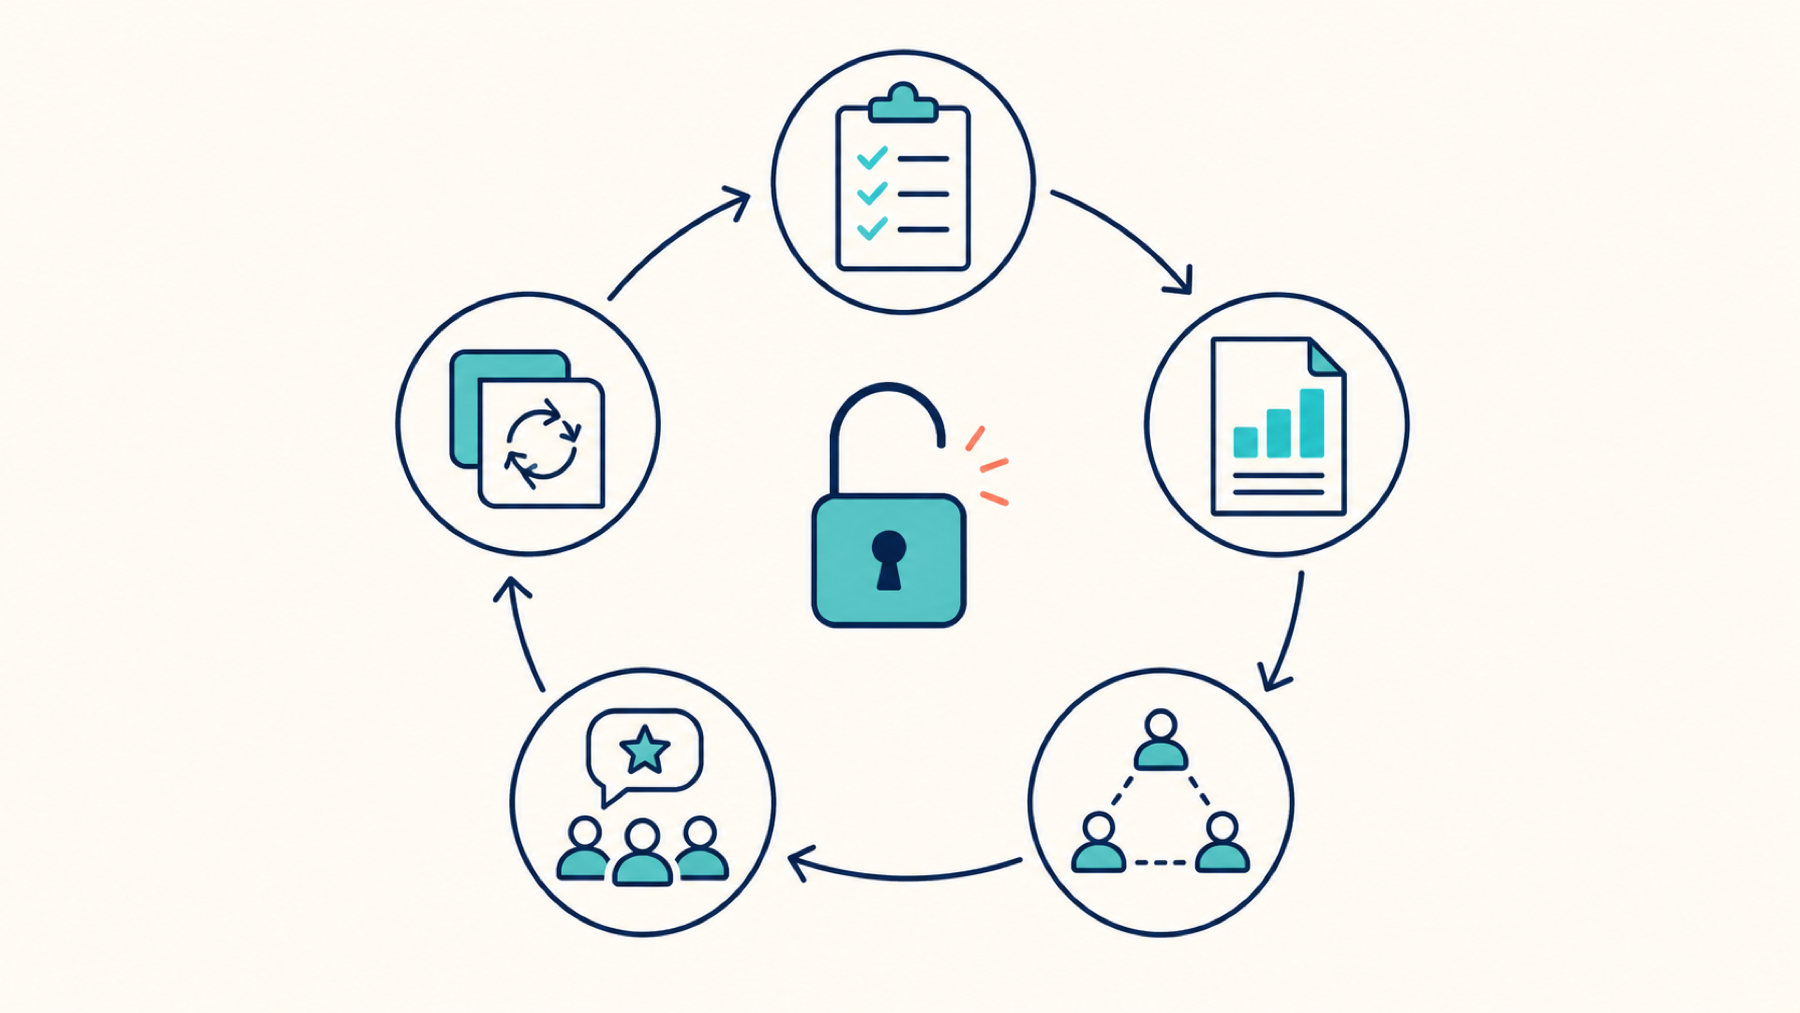
\includegraphics[width=\paperwidth,height=\paperheight]{assets/open-science-hero.png}};
    \fill[Warm,opacity=.94] (current page.south west) rectangle ([xshift=7.25cm]current page.north west);
    \fill[Teal] (current page.south west) rectangle ([xshift=.16cm]current page.north west);
    \node[anchor=south east] at ([xshift=-.34cm,yshift=.34cm]current page.south east)
      {\href{\ccLicenseURL}{
\includegraphics[width=.66cm]{assets/cc-by-nc-sa-4.0.png}}};
    \node[anchor=north east,fill=white,inner sep=3pt] at
      ([xshift=-.55cm,yshift=-.55cm]current page.north east)
      {\href{https://github.com/washingtonsegundo/open-science-presentation}{
\includegraphics[height=1.65cm]{assets/qr-github-repository.png}}};
  \end{tikzpicture}
  \vspace{0.65cm}
  \begin{minipage}{0.7\textwidth}
    \tagline{Apertura desde el diseño}\par
    \vspace{0.25cm}
    {\fontsize{24}{27}\selectfont\bfseries\color{Navy}Ciencia abierta}
    \vspace{0.2cm}

    {\usebeamerfont{subtitle}\color{Ink}Infraestructura abierta para una cooperación equitativa}
    \vspace{0.42cm}

    \small\color{Muted}Cómo la infraestructura pública brasileña puede impulsar una agenda compartida de ciencia abierta en el Sur Global.
    \vspace{0.48cm}

    {\normalsize\bfseries\color{Navy}Washington Segundo}\par
    \vspace{0.10cm}
    {\small\color{Ink}Coordinador general de Información Científica y Técnica}\par
    \vspace{0.08cm}
    {\scriptsize\color{Muted}Instituto Brasileño de Información en Ciencia y Tecnología}\par
    {\scriptsize\color{Muted}Ministerio de Ciencia, Tecnología e Innovación}
  \end{minipage}
\end{frame}}

% Slide 2
\begin{frame}{La ciencia abierta transforma todo el ciclo de investigación}
  \begin{columns}[T,onlytextwidth]
    \column{.52\textwidth}
      \begin{center}\resizebox{.90\linewidth}{!}{\OpenScienceCycleDiagram}\end{center}
    \column{.44\textwidth}
      \vspace{0.18cm}
      \tagline{Un cambio de paradigma}
      \vspace{0.22cm}
      \begin{itemize}\setlength\itemsep{0.22cm}
        \item La apertura comienza en la planificación, antes de publicar.
        \item Publicaciones, datos, código, métodos y revisiones son resultados reutilizables.
        \item La gobernanza, la preservación y la participación forman parte de la calidad científica.
      \end{itemize}
      \vspace{0.22cm}
      \colorbox{Mist}{\parbox{.93\linewidth}{\small\textbf{Idea central:} el conocimiento debe ser accesible, auditable, interoperable y útil para la sociedad.}}
  \end{columns}
\end{frame}

% Slide 3
\begin{frame}{Del intercambio privado a los ecosistemas abiertos}
  \vspace{0.3cm}
  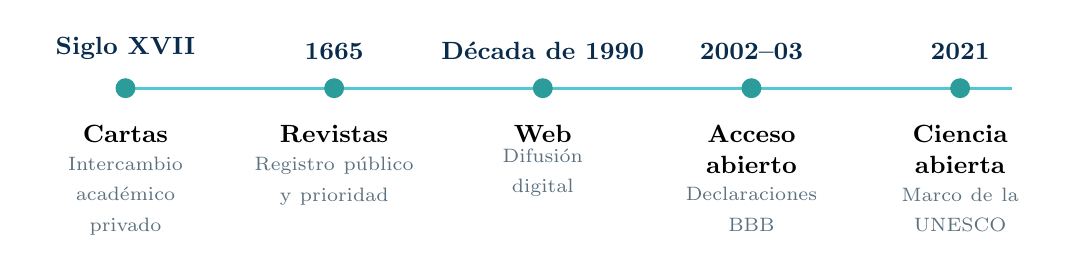
\begin{tikzpicture}[x=2.65cm,y=1cm]
    \draw[very thick,Cyan] (0,0) -- (4.25,0);
    \foreach \x/\yr/\head/\copy in {
      0/Siglo XVII/Cartas/Intercambio académico privado,
      1/1665/Revistas/Registro público y prioridad,
      2/Década de 1990/Web/Difusión\\digital,
      3/2002--03/Acceso abierto/Declaraciones BBB,
      4/2021/Ciencia abierta/Marco de la UNESCO}
    {
      \fill[Teal] (\x,0) circle (3.6pt);
      \node[above=7pt,align=center,text=Navy,font=\bfseries\small] at (\x,0) {\yr};
      \node[below=10pt,align=center,text width=2.25cm,font=\small] at (\x,0) {\textbf{\head}\\[-1pt]{\scriptsize\color{Muted}\copy}};
    }
  \end{tikzpicture}
  \vfill
  \begin{center}\colorbox{Mist}{\parbox{.88\linewidth}{\centering\small Las redes digitales separaron las funciones tradicionales de las revistas: registro, certificación, difusión y preservación.}}\end{center}
\end{frame}

% Slide 4
\begin{frame}{Ibict ha impulsado la información científica}
  \begin{columns}[T,onlytextwidth]
    \column{.30\textwidth}
      \vspace{0.10cm}
      \begin{center}
        {\fontsize{42}{46}\selectfont\bfseries\color{Teal}1954}
        \vspace{0.18cm}

        {\small\color{Muted}Fundado como instituto nacional de Brasil dedicado a la bibliografía y la documentación científica}
      \end{center}
      \vspace{0.25cm}
      \colorbox{Mist}{\parbox{.90\linewidth}{\centering\small\textbf{Hoy}\par Unidad de investigación del Ministerio de Ciencia, Tecnología e Innovación (MCTI)}}
    \column{.66\textwidth}
      \tagline{Una misión pública de larga trayectoria}
      \vspace{0.24cm}
      \begin{itemize}\setlength\itemsep{0.32cm}
        \item Organizar, preservar y difundir la información científica y tecnológica de Brasil.
        \item Desarrollar servicios nacionales, estándares e infraestructuras de información interoperables.
        \item Conectar la investigación brasileña con redes regionales e internacionales de conocimiento.
      \end{itemize}
      \vspace{0.22cm}
      \tagline{Una sólida tradición de apertura}\par
      \vspace{0.20cm}
      \small Ibict mantiene un papel de liderazgo en \textbf{Acceso Abierto} y \textbf{Ciencia Abierta}, impulsando repositorios, agregadores, datos de investigación, preservación digital, identificadores persistentes y gobernanza de interés público.
  \end{columns}
\end{frame}

% Slide 5
\begin{frame}{Cuatro ejes convierten la información en valor público}
  \vspace{0.08cm}
  \begin{columns}[T,onlytextwidth]
    \column{.49\textwidth}
      \keypoint{Integridad y justicia informacional}{Preservar la autoría y el significado en el ciclo de la información, con equidad en su producción, acceso y uso.}
      \vspace{0.28cm}

      \keypoint{Información para la ciudadanía}{Desarrollar alfabetización crítica, mediática y de datos para un entorno informacional multilingüe, accesible e inclusivo.}
    \column{.49\textwidth}
      \keypoint{Soberanía informacional}{Reforzar el control público de los flujos de información, infraestructuras, algoritmos, estándares, software y hardware.}
      \vspace{0.28cm}

      \keypoint{Ciencia Abierta}{Las prácticas de investigación abiertas refuerzan la confianza pública, la cooperación y la diplomacia científica.}
  \end{columns}
  \vfill
  \begin{center}
    \small\alert{\textbf{La ciencia de la información conecta los cuatro ejes} para apoyar el desarrollo social, ambiental y económico.}

    \vspace{0.09cm}
    {\tiny Fuente: Braga, \textit{Ciência da Informação}, vol. 55, no. 1, 2026.}
  \end{center}
\end{frame}

% Slide 6
\begin{frame}{Infraestructuras abiertas, investigación y ODS}
\begin{columns}[T,onlytextwidth]\column{.48\textwidth}\keypoint{ODS 4: Educación de calidad}{Conocimiento abierto, educación, formación y desarrollo de capacidades.}\vspace{.06cm}\par\keypoint{ODS 9: Industria, innovación e infraestructura}{Sistemas públicos interoperables para la investigación y la innovación.}\vspace{.06cm}\par\keypoint{ODS 10: Reducción de las desigualdades}{Participación y visibilidad más equitativas entre comunidades.}\column{.48\textwidth}\keypoint{ODS 16: Paz, justicia e instituciones sólidas}{Evidencia para el seguimiento de políticas y la rendición de cuentas.}\vspace{.06cm}\par\keypoint{ODS 17: Alianzas para lograr los objetivos}{Estándares y herramientas compartidos y cooperación institucional.}\vspace{.06cm}\par\small Las tecnologías sociales vinculan la investigación con necesidades públicas definidas localmente.\end{columns}
\vfill
\begin{center}\small Vías propuestas de beneficio público cuyos resultados deberán evaluarse.\\[.08cm]{\tiny Fuente: \href{https://sdgs.un.org/goals}{Objetivos de Desarrollo Sostenible de las Naciones Unidas}.}\end{center}
\end{frame}

% Slide 7
\begin{frame}{\href{https://en.most.gov.cn/pressroom/202512/t20251219_195559.html}{El Sur Global convierte principios en acciones}}
  \vspace{0.05cm}
  \begin{center}
    \small\textbf{Principios compartidos:} igualdad y beneficio mutuo \quad $\vert$ \quad respeto por la diversidad

    \vspace{0.05cm}
    acceso universal \quad $\vert$ \quad colaboración abierta
  \end{center}
  \vspace{0.10cm}
  \begin{columns}[T,onlytextwidth]
    \column{.49\textwidth}
      \keypoint{1 \; Gobernanza global}{Impulsar los principios de la UNESCO con gobernanza y seguimiento conjuntos.}
      \vspace{0.04cm}
      \keypoint{2 \; Cooperación en datos abiertos}{Conectar plataformas para compartir de forma ética y sostenible.}
      \vspace{0.04cm}
      \keypoint{3 \; Infraestructura compartida}{Desarrollar juntos servicios públicos y espacios de datos confiables.}
    \column{.49\textwidth}
      \keypoint{4 \; Comunicación científica abierta}{Compartir artículos y preprints mediante infraestructuras inclusivas.}
      \vspace{0.04cm}
      \keypoint{5 \; Participación pública}{Impulsar la cultura, la educación, la comunicación y la participación.}
      \vspace{0.04cm}
      \keypoint{6 \; Capacidades en países en desarrollo}{Desarrollar capacidades mediante intercambios y tecnología abierta.}
  \end{columns}
\end{frame}

% Slide 8
\begin{frame}{El ecosistema va más allá del acceso abierto}
  \vspace{0.15cm}
  \begin{columns}[T,onlytextwidth]
    \column{.49\textwidth}
      \keypoint{Resultados abiertos}{Publicaciones, datos de investigación, software, métodos y recursos educativos.}
      \vspace{0.28cm}

      \keypoint{Procesos abiertos}{Preprints, revisión por pares transparente, evaluación responsable y flujos reproducibles.}
    \column{.49\textwidth}
      \keypoint{Infraestructuras abiertas}{Repositorios, identificadores, estándares de metadatos, preservación y sistemas de información de investigación.}
      \vspace{0.28cm}

      \keypoint{Participación abierta}{Ciencia ciudadana, diálogo de saberes, inclusión y participación pública.}
  \end{columns}
  \vfill
  \begin{center}\alert{La infraestructura conecta todos los pilares y sostiene la apertura.}\end{center}
\end{frame}

% Slide 9
\begin{frame}{Cuatro principios equilibran calidad técnica y responsabilidad social}
  \begin{columns}[T,onlytextwidth]
    \column{.49\textwidth}
      \keypoint{FAIR}{Hacer los datos localizables, accesibles, interoperables y reutilizables para personas y máquinas.}
      \vspace{0.28cm}

      \keypoint{CARE}{Proteger el beneficio colectivo, la autoridad, la responsabilidad y la ética en la gobernanza de datos.}
    \column{.49\textwidth}
      \keypoint{TRUST}{Crear infraestructuras transparentes, responsables, centradas en los usuarios, sostenibles y técnicamente sólidas.}
      \vspace{0.28cm}

      \keypoint{DEIA}{Incorporar diversidad, equidad, inclusión y accesibilidad en los sistemas de investigación.}
  \end{columns}
  \vfill
  \begin{center}\small\textbf{Principio orientador:} tan abierto como sea posible, tan cerrado como sea necesario.\end{center}

  \begin{center}\alert{Maximizar la apertura con eficacia, estrategia, inclusión y responsabilidad}\end{center}

\end{frame}

% Slide 10
\begin{frame}{La publicación abierta debe cerrar la brecha de información científica}
  \small
  \begin{tabular}{@{}>{\raggedright\arraybackslash}p{2.15cm}>{\raggedright\arraybackslash}p{3.0cm}>{\raggedright\arraybackslash}p{3.35cm}>{\raggedright\arraybackslash}p{3.25cm}@{}}
    \toprule
    \textbf{Vía} & \textbf{Cómo ofrece \mbox{acceso}} & \textbf{Principal ventaja} & \textbf{Principal riesgo} \\
    \midrule
    Verde & Depósito en un \mbox{repositorio} & Utiliza infraestructura pública & Embargos o políticas editoriales restrictivas \\
    \addlinespace[0.14cm]
    Dorada & Acceso inmediato en la plataforma editorial & Versión publicada en abierto & Los cargos por publicación (APC) pueden excluir autores \\
    \addlinespace[0.14cm]
    Diamante & Sin cargos para lectores ni autores & Alinea la publicación con el interés público & Financiación y gobernanza sostenidas \\
    \bottomrule
  \end{tabular}
  \vfill
  \begin{center}
    \colorbox{Mist}{\parbox{.92\linewidth}{\centering\small La publicación diamante necesita financiación sostenida, gobernanza compartida y estándares editoriales sólidos.}}
  \end{center}
\end{frame}

% Slide 11
\begin{frame}{Publicar, revisar y curar: el potencial de los preprints}
  \begin{columns}[T,onlytextwidth]
    \column{.31\textwidth}
      \keypoint{1. Publicar}{Compartir un preprint temprano, con identificador persistente e historial de versiones claro.}
    \column{.31\textwidth}
      \keypoint{2. Revisar}{Invitar a la evaluación crítica y facilitar el acceso a las revisiones y respuestas de autores.}
    \column{.31\textwidth}
      \keypoint{3. Curar}{Seleccionar, contextualizar y recomendar trabajos con criterios editoriales transparentes.}
  \end{columns}
  \vspace{.35cm}
  \begin{itemize}\setlength\itemsep{.16cm}
    \item El acceso temprano puede acelerar los comentarios, la colaboración y la reutilización.
    \item Vincular preprints, revisiones, versiones corregidas y publicaciones en revistas.
    \item Indicar claramente el estado de revisión. La disponibilidad temprana no demuestra validez.
  \end{itemize}
  \vfill
  {\tiny Fuente: \href{https://publish-review-curate.org/}{COAR y ASAPbio, iniciativa Publish, Review, Curate}.}
\end{frame}

% Slide 12
\begin{frame}{La apertura también debe promover la justicia informacional}
  \begin{columns}[T,onlytextwidth]
    \column{.53\textwidth}
      \tagline{Tres dimensiones}
      \vspace{0.25cm}
      \begin{itemize}\setlength\itemsep{0.22cm}
        \item \textbf{Distribución:} acceso equitativo a la información y la infraestructura.
        \item \textbf{Reconocimiento:} respeto por la diversidad de personas, saberes y epistemologías.
        \item \textbf{Participación:} inclusión efectiva en la producción y el uso del conocimiento.
      \end{itemize}
    \column{.43\textwidth}
      \tagline{Salvaguardas éticas}
      \vspace{0.25cm}
      \begin{itemize}\setlength\itemsep{0.22cm}
        \item Consentimiento y evaluación de riesgos
        \item Privacidad y acceso controlado
        \item Derechos colectivos e indígenas sobre los datos
        \item Protección frente a usos perjudiciales o duales
      \end{itemize}
  \end{columns}
\end{frame}

% Slide 13
\begin{frame}{La implementación depende de la mediación humana}
  \small\begin{columns}[T,onlytextwidth]
    \column{.31\textwidth}
      \tagline{Diseño inclusivo}\par
      \vspace{0.23cm}
      \textbf{Diseñar para comunidades diversas}
      \vspace{0.16cm}
      \begin{itemize}\setlength\itemsep{0.22cm}
        \item Interfaces accesibles
        \item Búsqueda multilingüe
        \item Flexibilidad disciplinaria
        \item Flujos adaptados al contexto
      \end{itemize}
    \column{.31\textwidth}
      \tagline{Gobernanza}\par
      \vspace{0.23cm}
      \textbf{Definir responsabilidades}
      \vspace{0.16cm}
      \begin{itemize}\setlength\itemsep{0.22cm}
        \item Control de datos y privacidad
        \item Criterios de curación
        \item Salvaguardas éticas
        \item Responsabilidad institucional sostenible
      \end{itemize}
    \column{.31\textwidth}
      \tagline{Desarrollo de capacidades}\par
      \vspace{0.23cm}
      \textbf{Facilitar el uso crítico}
      \vspace{0.16cm}
      \begin{itemize}\setlength\itemsep{0.22cm}
        \item Educación y formación
        \item Límites e incertidumbre
        \item Prácticas reproducibles
        \item Reconocimiento de datos y software
      \end{itemize}
  \end{columns}
  \vfill
  \begin{center}\small\color{Muted}Reconocer el intercambio de datos, el software, la revisión y la curación. Los equipos de apoyo llevan los principios a la práctica.\end{center}
\end{frame}

% Slide 14
\begin{frame}{Brasil conecta servicios públicos en todo el ciclo de investigación}
\begin{columns}[T,onlytextwidth]\column{.48\textwidth}\tagline{Recolectar, publicar y conectar}\par\vspace{.20cm}
\begin{itemize}\setlength\itemsep{.22cm}
\item SciELO, revistas y repositorios institucionales
\item BDTD para la investigación de posgrado
\item Oasisbr para buscar en distintas colecciones
\end{itemize}
\column{.48\textwidth}\tagline{Integrar, identificar y preservar}\par\vspace{.20cm}
\begin{itemize}\setlength\itemsep{.22cm}
\item BrCris para conectar el sistema de investigación
\item Laguna para integrar datos heterogéneos
\item dARK para identificadores y Cariniana para preservación
\end{itemize}
\end{columns}
\vfill
\begin{center}\small Los estándares compartidos y la financiación estable apoyan la interoperabilidad y la autonomía institucional.\end{center}
\end{frame}

% Slide 15
\begin{frame}{Redes nacionales para la cooperación global}
  \begin{center}
  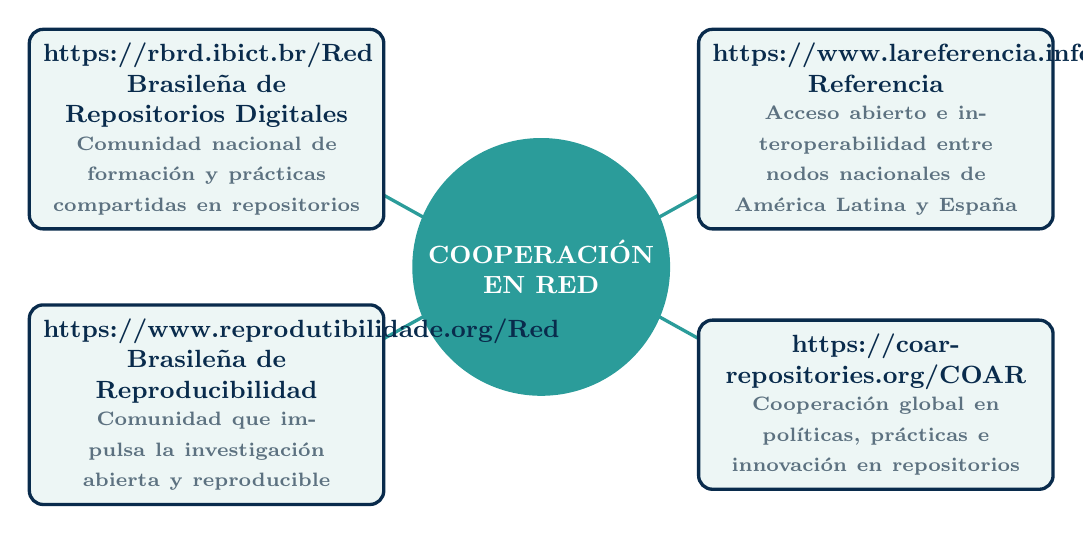
\begin{tikzpicture}[x=1cm,y=1cm]
    % Connections are drawn first so they remain behind the network nodes.
    \draw[diagram arrow] (-1.35,0.55) -- (-3.15,1.55);
    \draw[diagram arrow] (-1.35,-0.55) -- (-3.15,-1.55);
    \draw[diagram arrow] (1.35,0.55) -- (3.15,1.55);
    \draw[diagram arrow] (1.35,-0.55) -- (3.15,-1.55);

    \node[draw=Teal,very thick,circle,fill=Teal,text=white,align=center,
      minimum size=2.35cm,font=\bfseries\small] at (0,0)
      {COOPERACIÓN\\EN RED};

    \node[diagram node,text width=4.15cm,minimum height=1.52cm] at (-4.25,1.75)
      {\href{https://rbrd.ibict.br/}{\textbf{Red Brasileña de\\Repositorios Digitales}}\\[-1pt]
       {\scriptsize\color{Muted}Comunidad nacional de formación y prácticas compartidas en repositorios}};

    \node[diagram node,text width=4.15cm,minimum height=1.52cm] at (-4.25,-1.75)
      {\href{https://www.reprodutibilidade.org/}{\textbf{Red Brasileña de\\Reproducibilidad}}\\[-1pt]
       {\scriptsize\color{Muted}Comunidad que impulsa la investigación abierta y reproducible}};

    \node[diagram node,text width=4.15cm,minimum height=1.52cm] at (4.25,1.75)
      {\href{https://www.lareferencia.info/}{\textbf{LA Referencia}}\\[-1pt]
       {\scriptsize\color{Muted}Acceso abierto e interoperabilidad entre nodos nacionales de América Latina y España}};

    \node[diagram node,text width=4.15cm,minimum height=1.52cm] at (4.25,-1.75)
      {\href{https://coar-repositories.org/}{\textbf{COAR}}\\[-1pt]
       {\scriptsize\color{Muted}Cooperación global en políticas, prácticas e innovación en repositorios}};
  \end{tikzpicture}
  \end{center}
  \vspace{-0.10cm}
  \begin{center}
    \small\color{Muted}Las redes llevan a la práctica los objetivos 1 y 3 mediante estándares compartidos, aprendizaje y acción colectiva.
  \end{center}
\end{frame}

{\setbeamertemplate{footline}{}\setbeamertemplate{background}{}
% Slide 16
\begin{frame}[plain]
  \begin{tikzpicture}[remember picture,overlay]
    \node[anchor=center,inner sep=0] (laguna) at (current page.center)
      {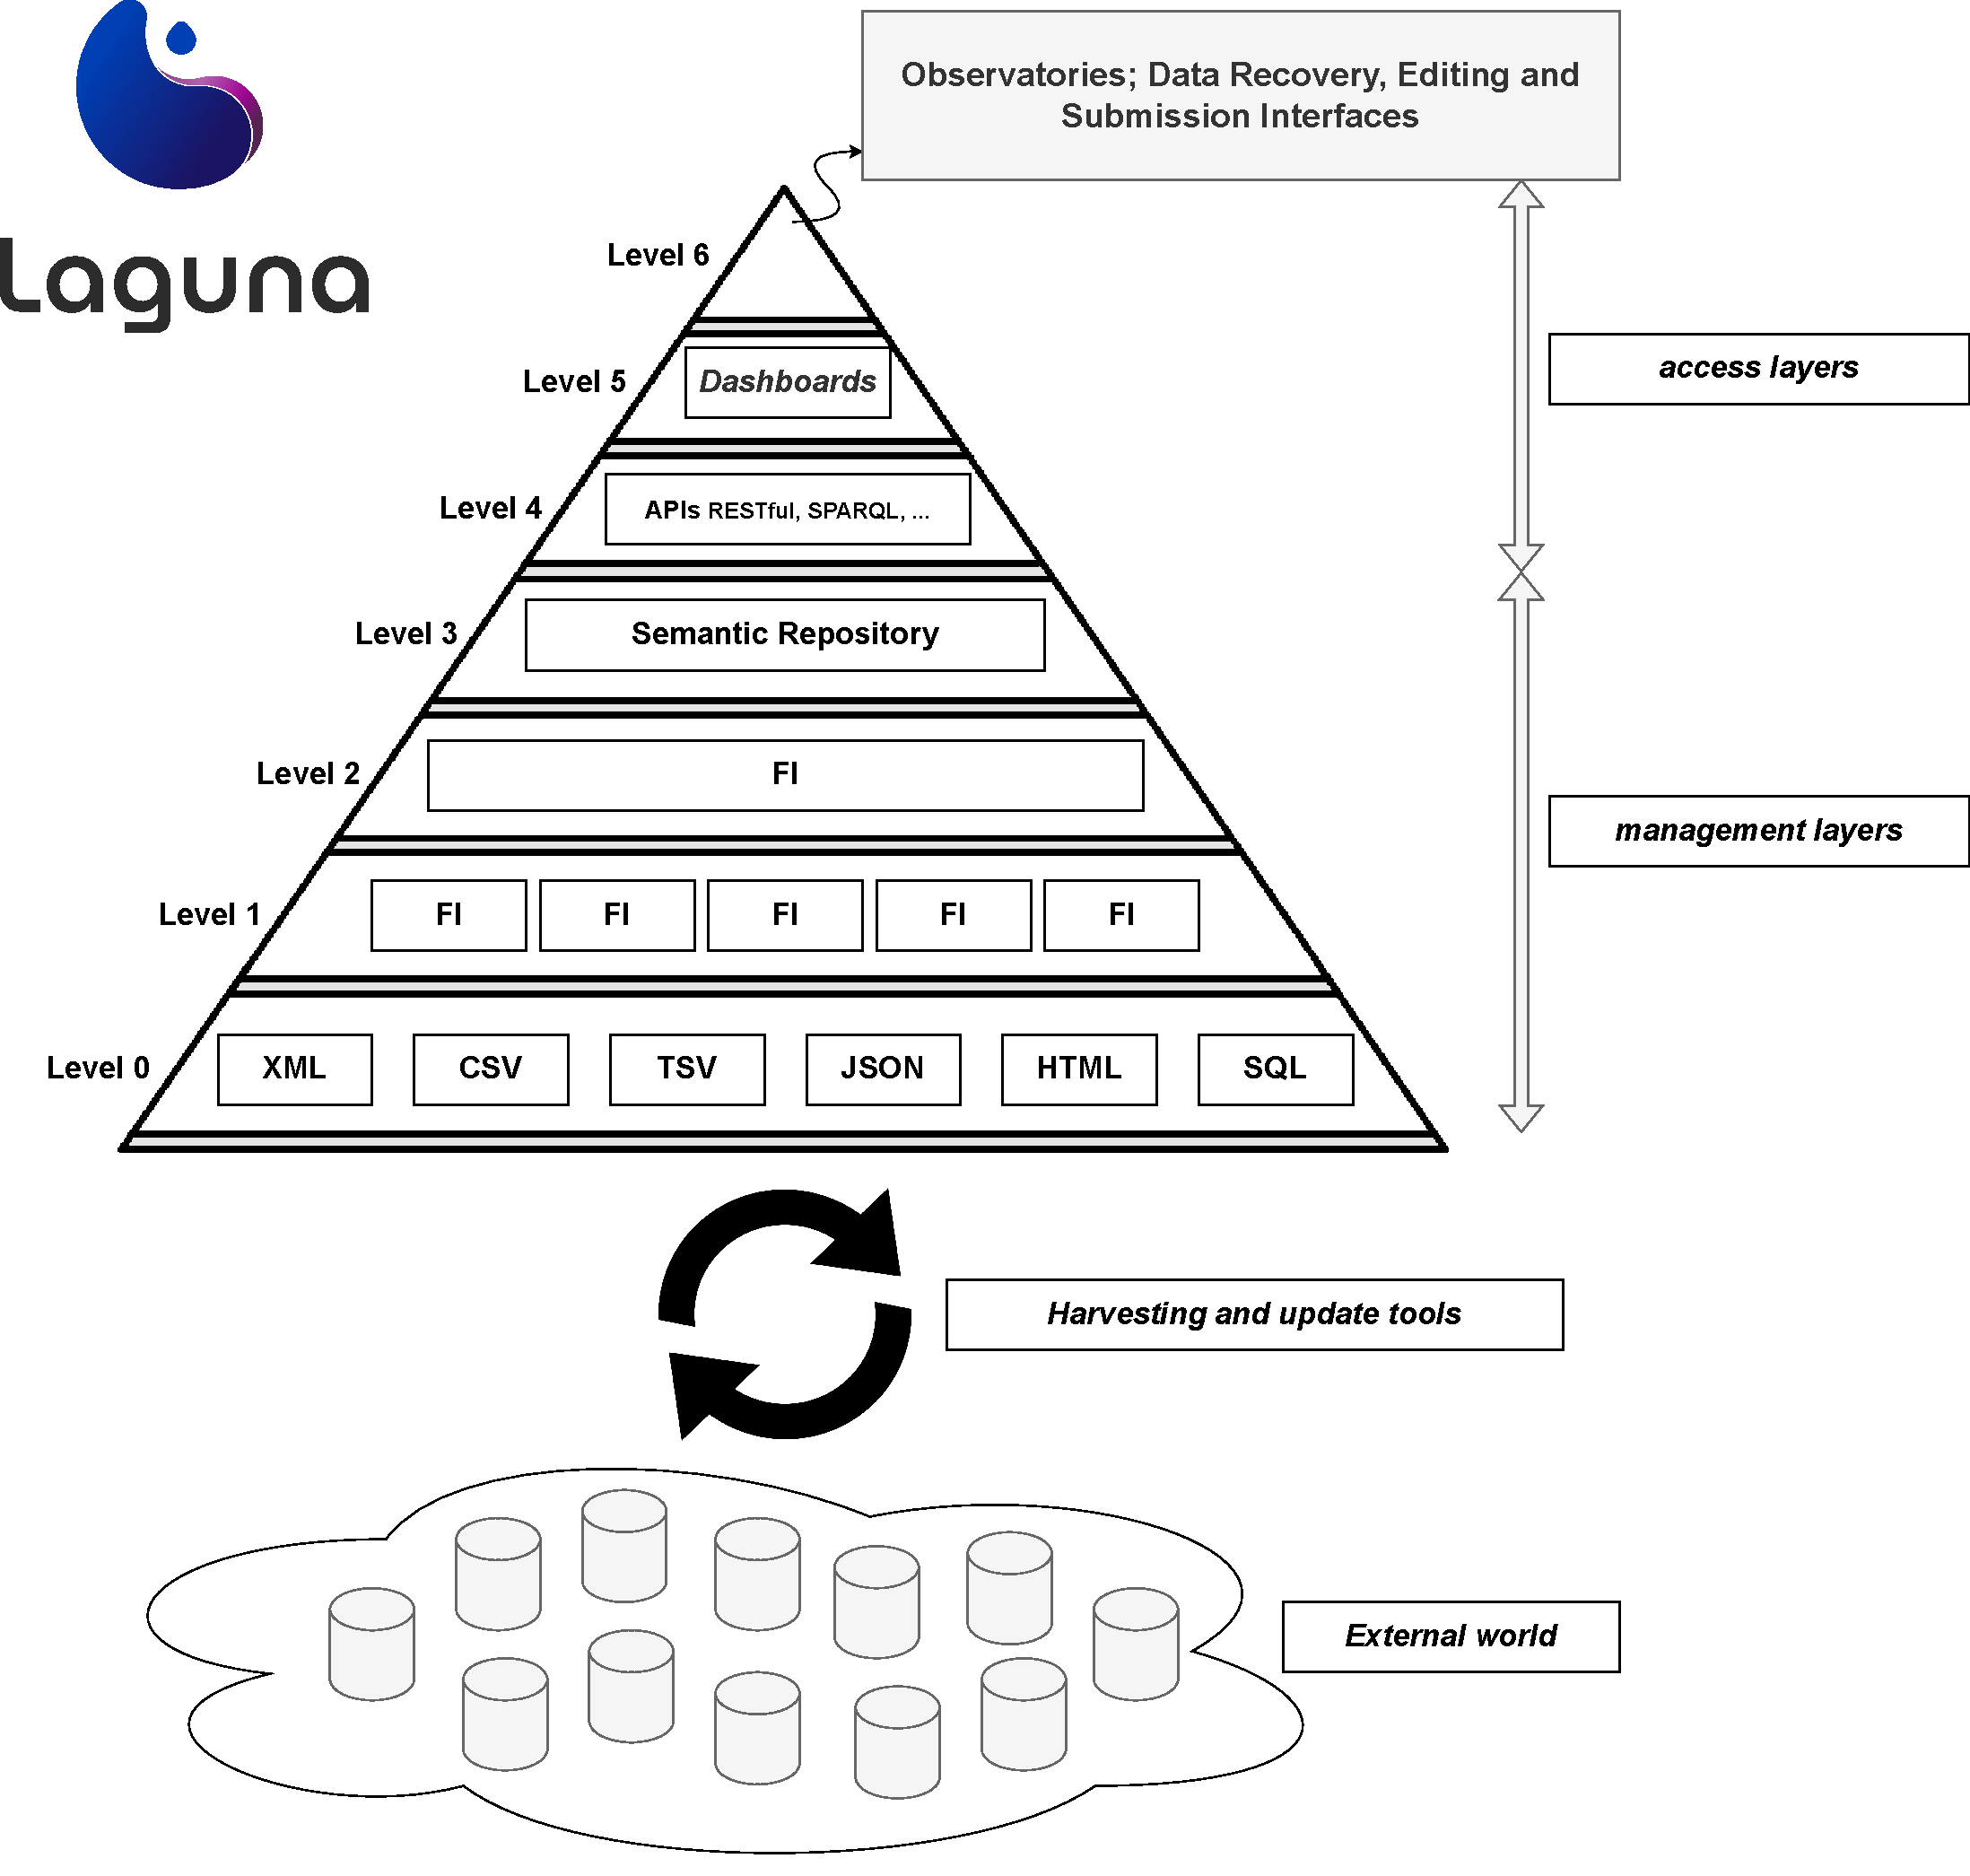
\includegraphics[height=.96\paperheight]{assets/laguna-architecture.pdf}};
    % Spanish labels over the original vector diagram; logos and topology retained.
    \path let \p1=(laguna.south west), \p2=(laguna.north east) in
      node[fill=white,text=black,font=\fontsize{6.3}{7}\selectfont\bfseries,align=center,minimum width=3.40cm,minimum height=.55cm] at ({\x1+.631*(\x2-\x1)},{\y1+.947*(\y2-\y1)}) {Observatorios e interfaces de recuperación,\\edición y envío de datos}
      node[fill=white,text=black,font=\fontsize{6.5}{7}\selectfont\bfseries,minimum width=.89cm,minimum height=.22cm] at ({\x1+.400*(\x2-\x1)},{\y1+.797*(\y2-\y1)}) {Paneles}
      node[fill=white,text=black,font=\fontsize{6.5}{7}\selectfont\bfseries,minimum width=2.0cm,minimum height=.23cm] at ({\x1+.398*(\x2-\x1)},{\y1+.662*(\y2-\y1)}) {Repositorio semántico}
      node[fill=white,text=black,font=\fontsize{6.5}{7}\selectfont\bfseries\itshape,minimum width=1.65cm,minimum height=.22cm] at ({\x1+.891*(\x2-\x1)},{\y1+.803*(\y2-\y1)}) {capas de acceso}
      node[fill=white,text=black,font=\fontsize{6.5}{7}\selectfont\bfseries\itshape,minimum width=1.65cm,minimum height=.22cm] at ({\x1+.891*(\x2-\x1)},{\y1+.558*(\y2-\y1)}) {capas de gestión}
      node[fill=white,text=black,font=\fontsize{6.3}{7}\selectfont\bfseries\itshape,minimum width=2.55cm,minimum height=.23cm] at ({\x1+.638*(\x2-\x1)},{\y1+.300*(\y2-\y1)}) {Herramientas de recolección y actualización}
      node[fill=white,text=black,font=\fontsize{6.5}{7}\selectfont\bfseries\itshape,minimum width=1.30cm,minimum height=.23cm] at ({\x1+.737*(\x2-\x1)},{\y1+.129*(\y2-\y1)}) {Mundo externo};
    \foreach \nx/\ny/\level in {.050/.430/0,.105/.512/1,.155/.586/2,.206/.662/3,.248/.729/4,.290/.797/5,.333/.864/6}{
      \path let \p1=(laguna.south west), \p2=(laguna.north east) in
      node[fill=white,text=black,font=\fontsize{6.5}{7}\selectfont\bfseries,inner sep=1pt,minimum width=.51cm,minimum height=.21cm] at ({\x1+\nx*(\x2-\x1)},{\y1+\ny*(\y2-\y1)}) {Nivel \level};
    }
    \node[anchor=south east,fill=white,inner sep=3pt] at
      ([xshift=-.34cm,yshift=.34cm]current page.south east)
      {\href{https://doi.org/10.21680/2447-7842.2023v9n2ID33825}{
\includegraphics[height=1.55cm]{assets/qr-doi-laguna.png}}};
  \end{tikzpicture}
\end{frame}}

% Slide 17
\begin{frame}{BrCris conecta el ecosistema brasileño de investigación}
\begin{columns}[T,onlytextwidth]\column{.52\textwidth}\tagline{Un sistema nacional de información de investigación}\par\vspace{.20cm}
\begin{itemize}\setlength\itemsep{.22cm}
\item Conectar investigadores, instituciones, proyectos y resultados.
\item Explorar relaciones para apoyar la gestión de la investigación.
\item Explorar nuevas opciones de interoperabilidad con OpenAlex y OpenCitations.
\end{itemize}
\small\color{Muted}15,9 millones de publicaciones: cifra de la plataforma en julio de 2026.\column{.44\textwidth}\vspace{.18cm}\href{https://brcris.ibict.br/}{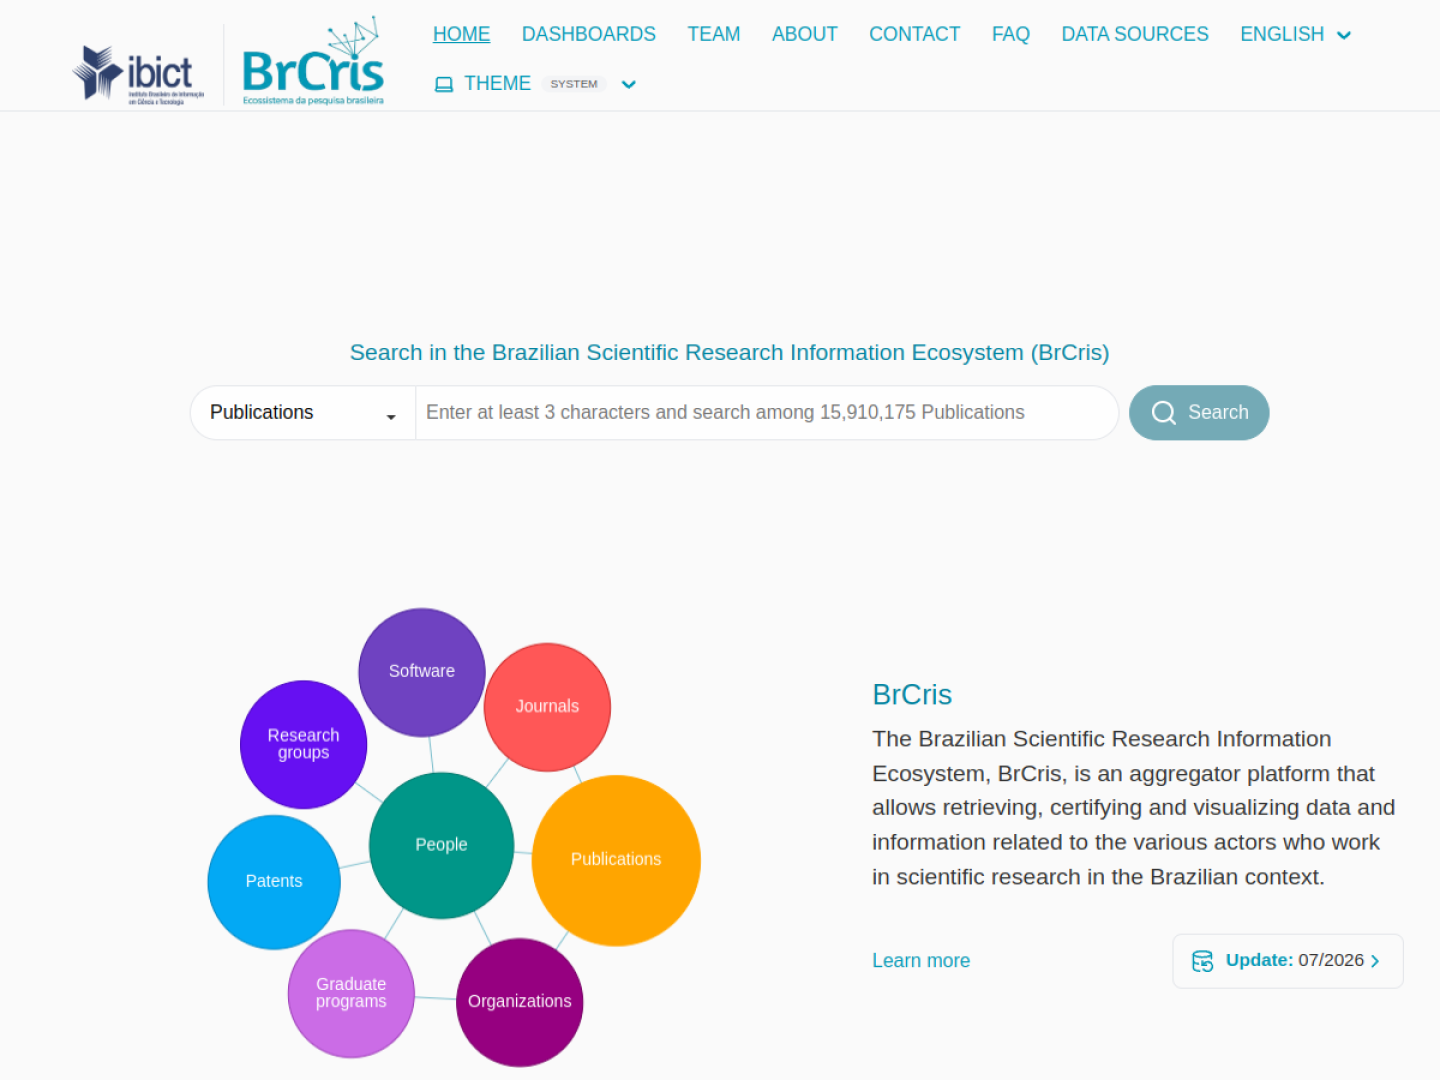
\includegraphics[width=\linewidth,trim=0 270 0 0,clip]{assets/screenshot-brcris.png}}\par\vspace{.20cm}\begin{minipage}[t]{.67\linewidth}\small Nuevas integraciones ofrecen oportunidades de cooperación por evaluar.\end{minipage}\hfill\begin{minipage}[t]{.28\linewidth}\vspace{0pt}\centering\href{https://brcris.ibict.br/}{
\includegraphics[width=\linewidth]{assets/qr-brcris.png}}\end{minipage}\end{columns}
\end{frame}

% Slide 18
\begin{frame}{Oasisbr conecta más de 6,5 millones de objetos digitales abiertos}
  \begin{columns}[T,onlytextwidth]
    \column{.43\textwidth}
      \vspace{0.04cm}
      \begin{center}
        \href{https://oasisbr.ibict.br/}{\begin{tikzpicture}
          \node[inner sep=0] (oasis) {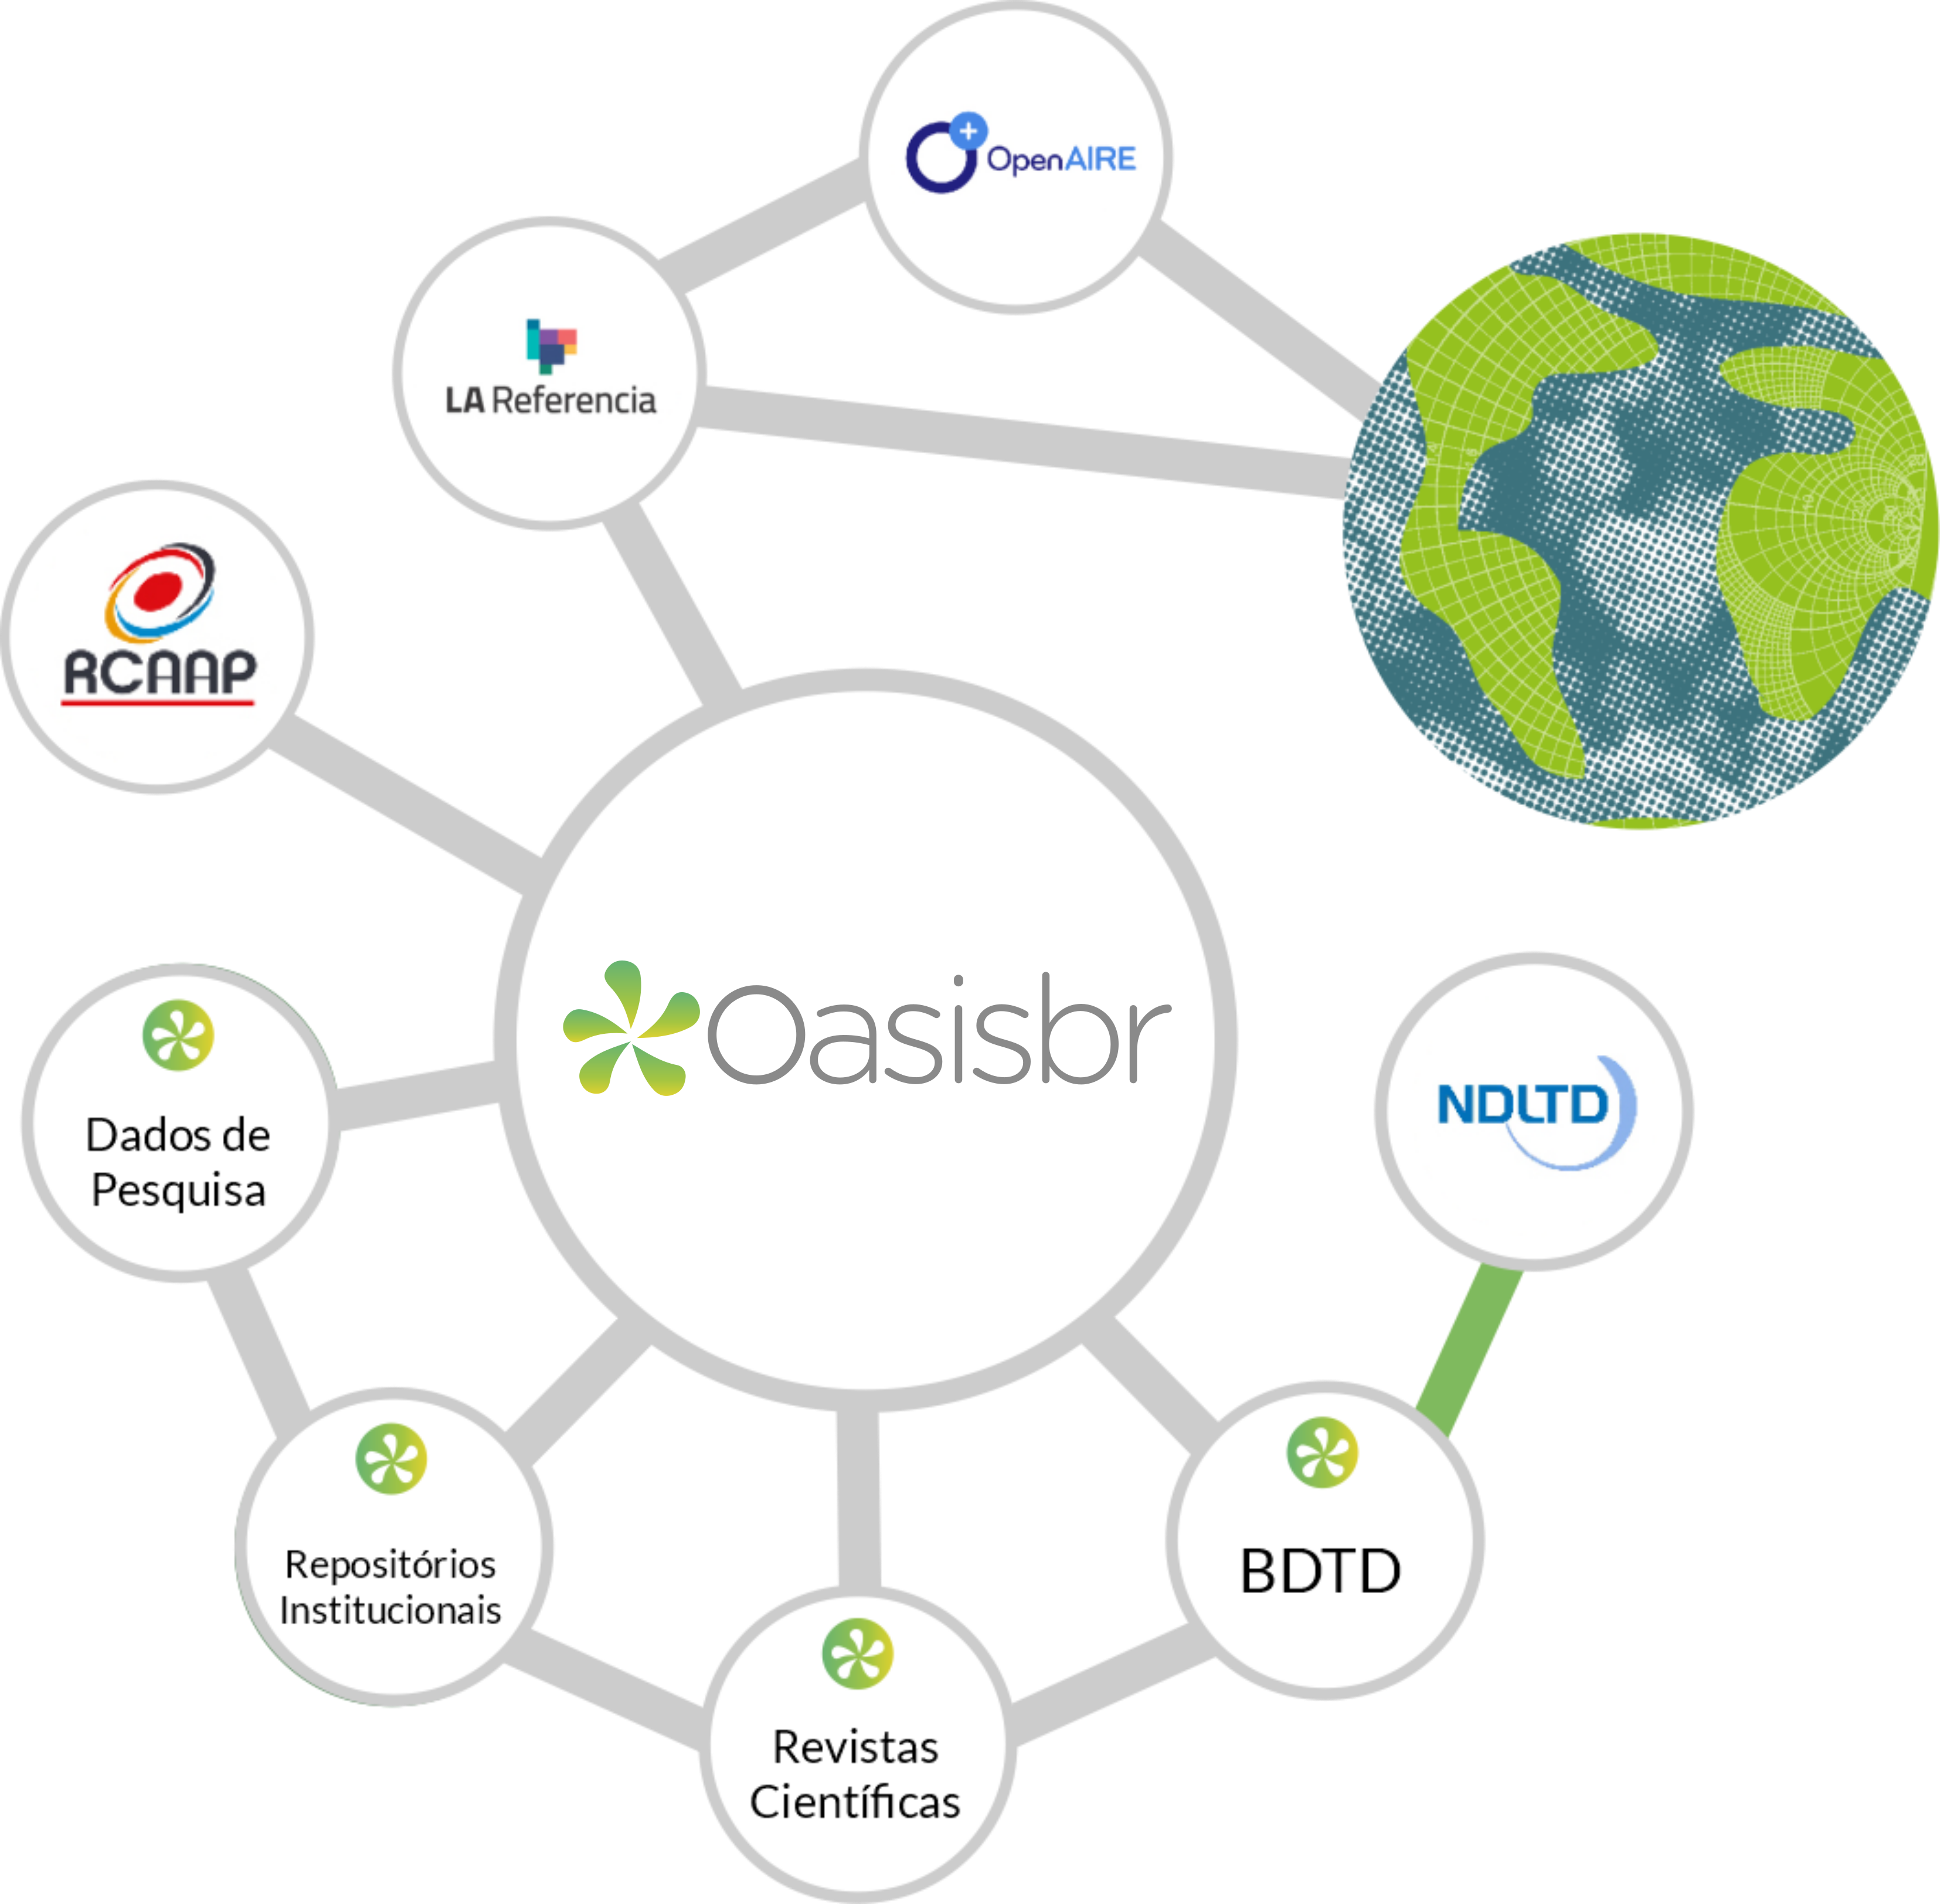
\includegraphics[height=.67\textheight]{assets/oasisbr-ecosystem.png}};
          \path let \p1=(oasis.south west), \p2=(oasis.north east) in
            node[fill=white,text=black,font=\fontsize{5.7}{6.3}\selectfont,align=center,inner sep=1pt,minimum width=.60cm,minimum height=.32cm] at ({\x1+.092*(\x2-\x1)},{\y1+.389*(\y2-\y1)}) {Datos de\\investigación}
            node[fill=white,text=black,font=\fontsize{5.7}{6.3}\selectfont,align=center,inner sep=1pt,minimum width=.73cm,minimum height=.28cm] at ({\x1+.202*(\x2-\x1)},{\y1+.165*(\y2-\y1)}) {Repositorios\\institucionales}
            node[fill=white,text=black,font=\fontsize{5.7}{6.3}\selectfont,align=center,inner sep=1pt,minimum width=.70cm,minimum height=.29cm] at ({\x1+.445*(\x2-\x1)},{\y1+.064*(\y2-\y1)}) {Revistas\\científicas};
        \end{tikzpicture}}
      \end{center}
    \column{.43\textwidth}
      \tagline{Una puerta de acceso nacional e internacional}
      \vspace{0.16cm}

      {\fontsize{28}{31}\selectfont\bfseries\color{Navy}6,5M+}\par
      {\small\color{Muted}artículos, tesis doctorales y de maestría, libros, capítulos y conjuntos de datos de investigación}
      \vspace{0.22cm}

      {\Large\bfseries\color{Teal}\raisebox{0.05ex}{$\sim$}1,2M}\par
      {\small\color{Muted}documentos agregados a través de BDTD}
      \vspace{0.22cm}

      {\Large\bfseries\color{Coral}\raisebox{0.05ex}{$\sim$}2.000}\par
      {\small\color{Muted}fuentes de información: repositorios y revistas científicas de Brasil}
    \column{.10\textwidth}
  \end{columns}
  \serviceqr{https://oasisbr.ibict.br/}{assets/qr-oasisbr.png}
\end{frame}

% Slide 19
\begin{frame}{BDTD da visibilidad a la investigación de posgrado}
  \small\begin{columns}[T,onlytextwidth]
    \column{.53\textwidth}
      \tagline{Un servicio nacional desde 2002}
      \vspace{0.22cm}
      \begin{itemize}\setlength\itemsep{0.18cm}
        \item Concebido, desarrollado y mantenido por Ibict.
        \item Integra tesis doctorales y de maestría de instituciones brasileñas de enseñanza e investigación.
        \item También incluye registros de trabajos defendidos por brasileños en instituciones del exterior.
        \item Ofrece búsqueda nacional gratuita. Las instituciones participantes alojan los textos completos.
      \end{itemize}
    \column{.35\textwidth}
      \tagline{Valor público}
      \vspace{0.22cm}
      \begin{itemize}\setlength\itemsep{0.18cm}
        \item Visibilidad de la investigación de posgrado
        \item Estándares comunes de metadatos
        \item Interoperabilidad institucional
        \item Acceso al conocimiento especializado
        \item Rendición de cuentas de la inversión pública
      \end{itemize}
    \column{.08\textwidth}
  \end{columns}
  \serviceqr{https://bdtd.ibict.br/}{assets/qr-bdtd.png}
\end{frame}

% Slide 20
\begin{frame}{dARK une identificación persistente y gobernanza compartida}
\begin{columns}[T,onlytextwidth]\column{.48\textwidth}\tagline{Responsabilidad institucional}\par\vspace{.20cm}
\begin{itemize}\setlength\itemsep{.22cm}
\item Identificadores descentralizados basados en ARK
\item Registros trazables y funciones operativas compartidas
\item Gobernanza, financiación y mantenimiento previstos desde el inicio
\end{itemize}
\column{.48\textwidth}\href{https://www.dark-pid.net/}{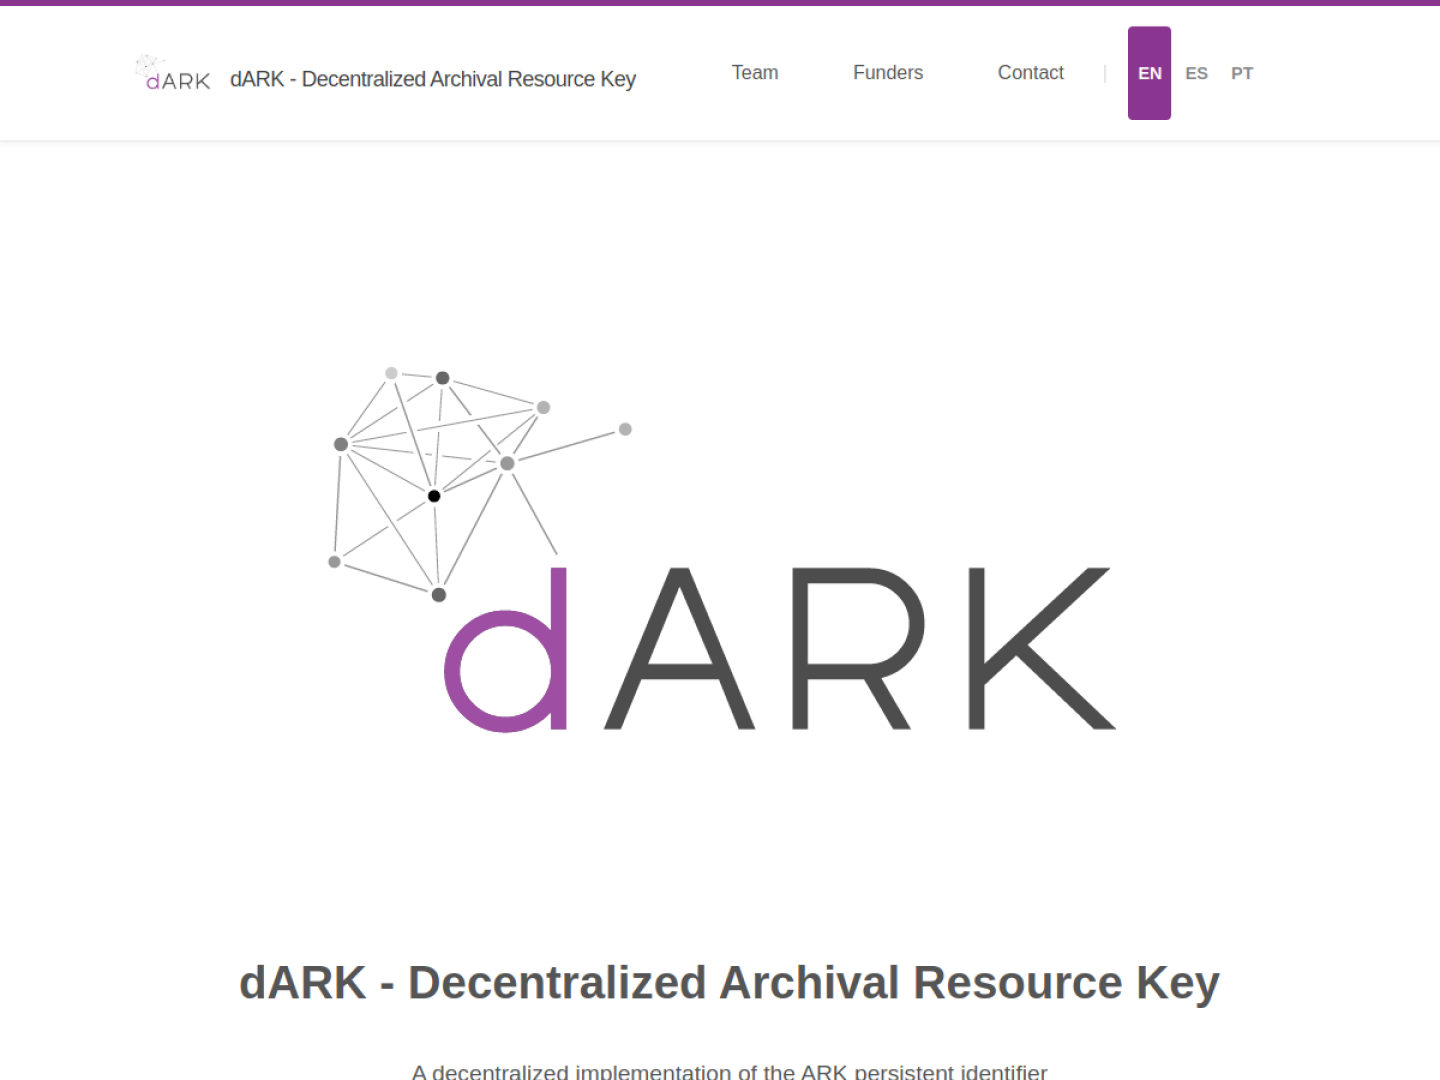
\includegraphics[width=\linewidth,trim=0 270 0 0,clip]{assets/screenshot-dark.png}}\par\small Colaboración con LA Referencia, con apoyo de Invest in Open Infrastructure.\end{columns}
\vfill
\noindent\begin{minipage}{.84\textwidth}\centering\small La identificación facilita la trazabilidad. La preservación mantiene disponibles los recursos.\end{minipage}
\serviceqr{https://www.dark-pid.net/}{assets/qr-dark.png}
\end{frame}

% Slide 21
\begin{frame}{La ciencia de la información sustenta una IA confiable}
  \begin{center}\resizebox{.94\linewidth}{!}{\KnowledgeValueChainDiagram}\end{center}
  \vspace{-0.08cm}

  \begin{columns}[T,onlytextwidth]
    \column{.32\textwidth}\centering
      \textbf{Ciencia de la información}\\[-1pt]
      {\scriptsize\color{Muted}Organiza, cura, representa y media el conocimiento}
    \column{.32\textwidth}\centering
      \textbf{Ciencia de datos}\\[-1pt]
      {\scriptsize\color{Muted}Analiza patrones, modela fenómenos y extrae valor}
    \column{.32\textwidth}\centering
      \textbf{Inteligencia artificial}\\[-1pt]
      {\scriptsize\color{Muted}Automatiza la cognición, la predicción y la interacción lingüística}
  \end{columns}
\end{frame}

% Slide 22
\begin{frame}{Una IA confiable requiere infraestructura de investigación confiable}
  \begin{center}\resizebox{.90\linewidth}{!}{\OpenInfrastructureDiagram}\end{center}
  \vspace{0.18cm}
  \begin{center}\small\color{Muted}La preservación y la interoperabilidad convierten los objetos almacenados en evidencia reutilizable y permiten los espacios de datos confiables y las aplicaciones de IA del objetivo 3.\end{center}
\end{frame}

% Slide 23
\begin{frame}{Los sistemas semánticos conectan significados y palabras clave}
  \begin{columns}[T,onlytextwidth]
    \column{.58\textwidth}
      \tagline{Recuperación basada en evidencia}\par
      \vspace{0.35cm}
      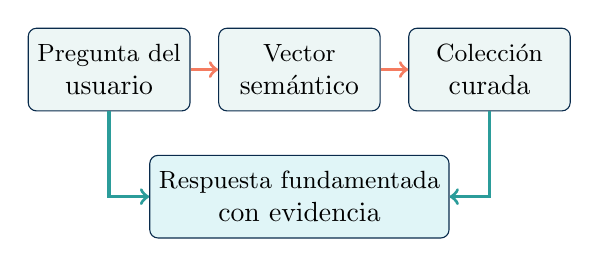
\begin{tikzpicture}[node distance=.25cm, every node/.style={align=center}]
        \node[draw=Navy,rounded corners=3pt,fill=Mist,minimum width=2.05cm,minimum height=1.05cm] (q) {\small Pregunta del\\usuario};
        \node[draw=Navy,rounded corners=3pt,fill=Mist,minimum width=2.05cm,minimum height=1.05cm,right=.35cm of q] (e) {\small Vector\\semántico};
        \node[draw=Navy,rounded corners=3pt,fill=Mist,minimum width=2.05cm,minimum height=1.05cm,right=.35cm of e] (r) {\small Colección\\curada};
        \draw[very thick,->,Coral] (q) -- (e);
        \draw[very thick,->,Coral] (e) -- (r);
        \node[draw=Navy,rounded corners=3pt,fill=Cyan!18,minimum width=3.05cm,minimum height=1.05cm,below=.55cm of e] (a) {\small Respuesta fundamentada\\con evidencia};
        \draw[very thick,->,Teal] (r.south) |- (a.east);
        \draw[very thick,->,Teal] (q.south) |- (a.west);
      \end{tikzpicture}
    \column{.38\textwidth}
      \tagline{Qué lo hace posible}
      \vspace{0.22cm}
      \begin{itemize}\setlength\itemsep{0.28cm}
        \item Los vocabularios controlados y las ontologías reducen la ambigüedad.
        \item Los vectores multilingües recuperan conceptos entre idiomas.
        \item RAG vincula las respuestas con los documentos recuperados.
        \item Verificar fuentes, omisiones y respuestas inciertas.
      \end{itemize}
  \end{columns}
\end{frame}

% Slide 24
\begin{frame}{La IA aplicada aporta valor con una base de información preparada}
  \small
  \begin{tabular}{@{}>{\raggedright\arraybackslash}p{2.35cm}>{\raggedright\arraybackslash}p{3.15cm}>{\raggedright\arraybackslash}p{5.9cm}@{}}
    \toprule
    \textbf{Aplicación} & \textbf{Capacidad de IA} & \textbf{Valor de interés público} \\
    \midrule
    ServicesPI & Búsqueda semántica + PLN & Búsqueda en lenguaje natural en colecciones complejas de patentes \\
    \addlinespace[0.12cm]
    Patente.IA & Similitud de texto e imagen & Mayor detección de invenciones relacionadas y del estado de la técnica \\
    \addlinespace[0.12cm]
    RDAPP & PLN + recuperación semántica & Acceso estructurado y análisis de documentos de políticas públicas \\
    \addlinespace[0.12cm]
    SAVITS & BI + ML + LLM & Seguimiento y análisis de políticas de tecnologías sociales \\
    \bottomrule
  \end{tabular}
  \vfill
  \begin{center}\colorbox{Mist}{\parbox{.9\linewidth}{\centering\small El control público de modelos e infraestructura requiere formación, verificación de fuentes y supervisión humana.}}\end{center}
\end{frame}

% Slide 25
\begin{frame}{Ibict puede contribuir}
  \small
  \begin{columns}[T,onlytextwidth]
    \column{.49\textwidth}
      \tagline{Gobernanza, datos e infraestructura}
      \vspace{0.18cm}
      \begin{itemize}\setlength\itemsep{0.25cm}
        \item \textbf{1 \; Gobernanza:} experiencia en políticas, redes, estándares y seguimiento.
        \item \textbf{2 \; Datos abiertos:} Oasisbr, BDTD, agregación de metadatos e interoperabilidad.
        \item \textbf{3 \; Infraestructura:} BrCris, Laguna, Cariniana, dARK y servicios digitales públicos.
      \end{itemize}
    \column{.49\textwidth}
      \tagline{Comunicación, participación y capacidades}
      \vspace{0.18cm}
      \begin{itemize}\setlength\itemsep{0.25cm}
        \item \textbf{4 \; Comunicación:} repositorios, revistas, publicación abierta y acceso persistente.
        \item \textbf{5 \; Participación:} alfabetización informacional, ciencia ciudadana y acceso multilingüe.
        \item \textbf{6 \; Capacidades:} formación, intercambio Sur--Sur y transferencia de tecnología abierta.
      \end{itemize}
  \end{columns}
  \vfill
  \begin{center}
    \colorbox{Mist}{\parbox{.90\linewidth}{\centering\small Brasil puede concretar los principios compartidos en servicios interoperables, capacidades profesionales y evidencia para la cooperación.}}

    \vspace{0.08cm}
    {\tiny\color{Muted}\href{https://en.most.gov.cn/pressroom/202512/t20251219_195559.html}{Vinculado al Plan de Acción para la Cooperación Internacional en Ciencia Abierta, 2025.}}
  \end{center}
\end{frame}

% Slide 26
\begin{frame}{La capacidad nacional hace posible la cooperación internacional}
  \begin{columns}[T,onlytextwidth]
    \column{.48\textwidth}
      \tagline{Base nacional}
      \vspace{0.20cm}
      \begin{itemize}\setlength\itemsep{0.20cm}
        \item Un punto focal que conecte socios nacionales e internacionales
        \item Funciones definidas para el gobierno, financiadores, instituciones y redes
        \item Financiación estable para infraestructuras públicas y equipos profesionales
        \item Estándares compartidos con adaptación regional y disciplinaria
      \end{itemize}
    \column{.48\textwidth}
      \tagline{Mecanismo multilateral}
      \vspace{0.20cm}
      \begin{itemize}\setlength\itemsep{0.20cm}
        \item Un mecanismo de intercambio con valor añadido definido
        \item Asignación coordinada de recursos y proyectos piloto concretos
        \item Seguimiento dinámico e informes transparentes
        \item Reuniones rotativas para compartir evidencia y mejorar las prácticas
      \end{itemize}
  \end{columns}
  \vfill
  \begin{center}\colorbox{Mist}{\parbox{.9\linewidth}{\centering\small Las instituciones nacionales sólidas sustentan la participación equitativa, las contribuciones conjuntas y los beneficios compartidos.}}\end{center}
\end{frame}

% Slide 27
\begin{frame}{Un piloto conjunto para políticas y evaluación justa de la investigación}
\begin{columns}[T,onlytextwidth]\column{.48\textwidth}\tagline{Seguimiento de políticas públicas}\par\vspace{.20cm}
\begin{itemize}\setlength\itemsep{.22cm}
\item Comenzar con políticas vinculadas a las tecnologías sociales.
\item Seguir la implementación, el alcance y los resultados comunicados.
\item Interpretar la evidencia con gestores y comunidades participantes.
\end{itemize}
\column{.48\textwidth}\tagline{Herramientas de evaluación científica}\par\vspace{.20cm}
\begin{itemize}\setlength\itemsep{.22cm}
\item Conectar repositorios, revistas y sistemas de información de investigación.
\item Documentar contribuciones diversas y su uso social.
\item Apoyar la evaluación contextual por investigadores y revisores.
\end{itemize}
\end{columns}
\vfill
\begin{center}\small Propuesta de diseño conjunto: acordar socios, responsabilidades, recursos, salvaguardas y calendario.\end{center}
\end{frame}

% Slide 28
\begin{frame}{La evidencia conectada apoya las políticas y la evaluación}
\small\begin{tabular}{@{}>{\raggedright\arraybackslash}p{3.4cm}>{\raggedright\arraybackslash}p{4.6cm}>{\raggedright\arraybackslash}p{4.6cm}@{}}\toprule\textbf{Evidencia por conectar} & \textbf{Herramienta propuesta} & \textbf{Uso por validar}\\\midrule Publicaciones, datos y software & Vínculos entre repositorios, revistas y registros de investigación & Rastrear contribuciones y reutilización entre resultados\\\addlinespace[.25cm]Documentos de políticas e informes de proyectos & Panel de seguimiento de políticas con enlaces a las fuentes & Examinar implementación, cobertura y vacíos de evidencia\\\addlinespace[.25cm]Revisiones y testimonios comunitarios & Portafolios de evidencia contextual para la revisión cualitativa & Examinar el uso social, la pertinencia local y distintas perspectivas\\\bottomrule\end{tabular}\vfill\begin{center}\small Comenzar con una muestra acordada. Documentar procedencia, permisos, incertidumbre y procedimientos de corrección.\end{center}
\end{frame}

% Slide 29
\begin{frame}{CoARA orienta una evaluación más justa de la investigación}
\begin{columns}[T,onlytextwidth]\column{.48\textwidth}\tagline{Principios de evaluación}\par\vspace{.20cm}
\begin{itemize}\setlength\itemsep{.22cm}
\item Reconocer resultados, actividades, funciones e idiomas diversos.
\item Priorizar el juicio cualitativo con revisión por pares.
\item Utilizar indicadores cuantitativos con responsabilidad y contexto.
\end{itemize}
\column{.48\textwidth}\tagline{Implicaciones para el piloto}\par\vspace{.20cm}
\begin{itemize}\setlength\itemsep{.22cm}
\item Evitar el uso inadecuado de métricas de revistas y del índice h.
\item Desarrollar criterios con investigadores y evaluadores.
\item Evaluar sesgos, transparencia y utilidad práctica de las herramientas.
\end{itemize}
\end{columns}
\vfill
\begin{center}\small {\footnotesize Coalición para el Avance de la Evaluación de la Investigación. Referencia para la propuesta, sin implicar adhesión institucional.}\\[.10cm]{\tiny Fuente: \href{https://www.coara.org/agreement/the-commitments/}{Compromisos de CoARA}, en particular 1--3, 6, 7 y 10.}\end{center}
\end{frame}

% Slide 30
\begin{frame}{¿Cómo reconoceríamos el éxito?}
\small\begin{tabular}{@{}>{\raggedright\arraybackslash}p{3.5cm}>{\raggedright\arraybackslash}p{5.2cm}>{\raggedright\arraybackslash}p{3.9cm}@{}}\toprule\textbf{Resultado esperado} & \textbf{Evidencia por recopilar} & \textbf{Pregunta de evaluación}\\\midrule Seguimiento útil de políticas & Uso documentado por gestores y comunidades & ¿La evidencia orientó la acción?\\\addlinespace[.22cm]Evaluación más inclusiva & Contribuciones reconocidas en diversos idiomas, funciones y resultados & ¿Qué trabajos ganaron visibilidad?\\\addlinespace[.22cm]Contribución social trazable & Casos de uso, testimonios y revisión contextual & ¿Qué cambió y para quién?\\\addlinespace[.22cm]Herramientas compartidas sostenibles & Reutilización, funciones de mantenimiento y capacidades demostradas & ¿Pueden los socios sostener el trabajo?\\\bottomrule\end{tabular}\vfill\begin{center}\small Acordar una línea de base y criterios antes del piloto. Evaluar la contribución a los resultados sin presuponer causalidad.\end{center}
\end{frame}

% Slide 31
\begin{frame}{Brasil puede concretar el plan en infraestructura compartida}
  \vspace{0.25cm}
  \begin{center}
  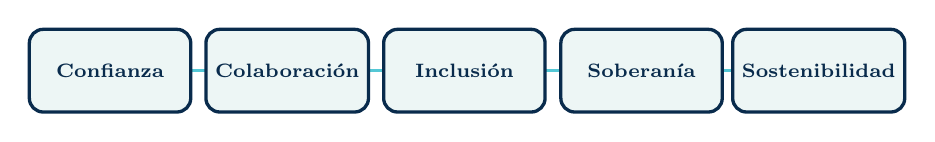
\begin{tikzpicture}[node distance=.35cm]
    \draw[very thick,Cyan] (0,0) -- (9,0);
    \foreach \name/\x/\label in {a/0/Confianza,b/2.25/Colaboración,c/4.5/Inclusión,d/6.75/Soberanía,e/9/Sostenibilidad}{
      \node[draw=Navy,very thick,fill=Mist,rounded corners=5pt,minimum width=2.05cm,
        minimum height=1.05cm,align=center,font=\bfseries\scriptsize,text=Navy] (\name) at (\x,0) {\label};
    }
  \end{tikzpicture}
  \end{center}
  \vspace{0.35cm}
  \begin{center}
    \Large\color{Navy}\textbf{Conectar servicios + iniciar pilotos + desarrollar capacidades + compartir evidencia}
  \end{center}
  \vspace{0.25cm}
  \begin{center}
    \normalsize\color{Muted}Ibict puede aportar servicios y alianzas para el seguimiento de políticas y una evaluación científica más justa, con el beneficio social como propósito común.
  \end{center}
  \vfill
 % \begin{center}\scriptsize\color{Muted}Condensed and translated from the supplied materials and official Ibict service websites, covering Ciencia Abierta, AI and data, Brazilian scientific information infrastructures, BrCris, Oasisbr, BDTD, the SDGs, national actions, and implementation pathways. Key frameworks referenced: UNESCO Ciencia Abierta Recommendation, FAIR, CARE, TRUST, DEIA, DORA, Leiden Manifesto, and CoARA.\end{center}
\end{frame}

% Slide 32
\begin{frame}{Comunidades de repositorios en Salvador, Brasil, en 2027}
  \vspace{-0.08cm}
  \begin{center}
    \href{https://or2027.openrepositories.org/}{
\includegraphics[width=.50\textwidth]{assets/openrepositories-logo.jpg}}
  \end{center}
  \vspace{-0.05cm}

  \begin{center}
  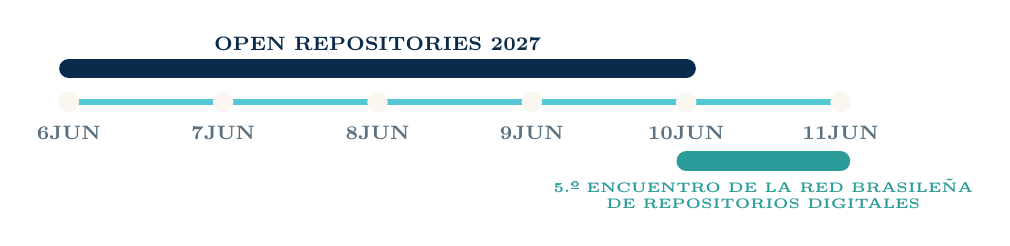
\begin{tikzpicture}[x=1cm,y=1cm]
    \draw[line width=2.2pt,Cyan] (0,0) -- (9.8,0);
    \foreach \x/\day in {0/6,1.96/7,3.92/8,5.88/9,7.84/10,9.8/11}{
      \fill[Warm] (\x,0) circle (3.7pt);
      \node[below=5pt,font=\scriptsize\bfseries,text=Muted] at (\x,0) {\day JUN};
    }
    \draw[line width=7pt,Navy,line cap=round] (0,.43) -- (7.84,.43);
    \node[above=3pt,font=\scriptsize\bfseries,text=Navy] at (3.92,.43) {OPEN REPOSITORIES 2027};
    \draw[line width=7pt,Teal,line cap=round] (7.84,-.75) -- (9.8,-.75);
    \node[below=3pt,align=center,font=\tiny\bfseries,text=Teal] at (8.82,-.75)
      {5.º ENCUENTRO DE LA RED BRASILEÑA\\DE REPOSITORIOS DIGITALES};
  \end{tikzpicture}
  \end{center}

  \vspace{-0.08cm}
  \begin{columns}[T,onlytextwidth]
    \column{.48\textwidth}
      {\footnotesize\bfseries\color{Teal}\MakeUppercase{6--10 de junio de 2027}}\par
      \vspace{0.10cm}

      {\normalsize\bfseries\color{Navy}Open Repositories 2027}\par
      \footnotesize\color{Muted}Salvador, Bahía: el intercambio global llega a la comunidad sudamericana de repositorios.
    \column{.48\textwidth}
      {\footnotesize\bfseries\color{Teal}\MakeUppercase{10--11 de junio de 2027}}\par
      \vspace{0.10cm}

      {\normalsize\bfseries\color{Navy}Red Brasileña de Repositorios}\par
      \footnotesize\color{Muted}El quinto encuentro nacional impulsa la cooperación y las prácticas compartidas en repositorios.
  \end{columns}
  \vspace{0.18cm}
  \begin{center}
    \small\bfseries\color{Teal}Una cita en 2027 para pilotos conjuntos, revisión de avances y coordinación de redes.
  \end{center}
\end{frame}

{\setbeamertemplate{footline}{}\setbeamertemplate{background}{}
% Slide 33
\begin{frame}[plain]
  \begin{tikzpicture}[remember picture,overlay]
    \fill[Teal] (current page.south west) rectangle ([xshift=.16cm]current page.north west);


    \node[font=\fontsize{30}{34}\selectfont\bfseries,text=Navy]
      at ([yshift=1.38cm]current page.center) {¡Gracias!};
    \node[font=\small\bfseries,text=Teal]
      at ([yshift=.55cm]current page.center) {washingtonsegundo@ibict.br};

    \node[align=center,text width=2.55cm,text=Navy] at ([xshift=-4.20cm,yshift=-.20cm]current page.center)
      {{\worldlatin\large Aguyjevete}\\[-1pt]\scriptsize\color{Muted}Guaraní};
    \node[align=center,text width=2.55cm,text=Navy] at ([xshift=-1.40cm,yshift=-.20cm]current page.center)
      {{\worldlatin\large Sulpayki}\\[-1pt]\scriptsize\color{Muted}Quechua};
    \node[align=center,text width=2.55cm,text=Navy] at ([xshift=1.40cm,yshift=-.20cm]current page.center)
      {{\worldlatin\large Asante}\\[-1pt]\scriptsize\color{Muted}Suajili / Bantú};
    \node[align=center,text width=2.55cm,text=Navy] at ([xshift=4.20cm,yshift=-.20cm]current page.center)
      {{\worldlatin\large Ngiyabonga}\\[-1pt]\scriptsize\color{Muted}Zulú / Bantú};

    \node[align=center,text width=2.55cm,text=Navy] at ([xshift=-4.20cm,yshift=-1.25cm]current page.center)
      {{\worldlatin\large Ẹ ṣé}\\[-1pt]\scriptsize\color{Muted}Yoruba};
    \node[align=center,text width=2.55cm,text=Navy] at ([xshift=-1.40cm,yshift=-1.25cm]current page.center)
      {{\worldlatin\large Na gode}\\[-1pt]\scriptsize\color{Muted}Hausa};
    \node[align=center,text width=2.55cm,text=Navy] at ([xshift=1.40cm,yshift=-1.25cm]current page.center)
      {{\devanagarifont\large धन्यवाद}\\[-1pt]\scriptsize\color{Muted}Hindi};
    \node[align=center,text width=2.55cm,text=Navy] at ([xshift=4.20cm,yshift=-1.25cm]current page.center)
      {{\bengalifont\large ধন্যবাদ}\\[-1pt]\scriptsize\color{Muted}Bengalí};

    \node[align=center,text width=2.20cm,text=Navy] at ([xshift=-4.80cm,yshift=-2.45cm]current page.center)
      {{\tamilfont\large நன்றி}\\[-1pt]\scriptsize\color{Muted}Tamil};
    \node[align=center,text width=2.20cm,text=Navy] at ([xshift=-2.40cm,yshift=-2.45cm]current page.center)
      {{\ethiopicfont\large አመሰግናለሁ}\\[-1pt]\scriptsize\color{Muted}Amárico};
    \node[align=center,text width=2.20cm,text=Navy] at ([yshift=-2.45cm]current page.center)
      {{\worldlatin\large Terima kasih}\\[-1pt]\scriptsize\color{Muted}Indonesio};
    \node[align=center,text width=2.20cm,text=Navy] at ([xshift=2.40cm,yshift=-2.45cm]current page.center)
      {{\chinesefont\large 谢谢}\\[-1pt]\scriptsize\color{Muted}Chino};
    \node[align=center,text width=2.20cm,text=Navy] at ([xshift=4.80cm,yshift=-2.45cm]current page.center)
      {{\worldlatin\large Obrigado}\\[-1pt]\scriptsize\color{Muted}Portugués};

    \node[anchor=south east] at ([xshift=-.34cm,yshift=.34cm]current page.south east)
      {\href{\ccLicenseURL}{
\includegraphics[width=.66cm]{assets/cc-by-nc-sa-4.0.png}}};
    \node[anchor=north east,fill=white,inner sep=3pt] at
      ([xshift=-.55cm,yshift=-.55cm]current page.north east)
      {\href{https://github.com/washingtonsegundo/open-science-presentation}{
\includegraphics[height=1.65cm]{assets/qr-github-repository.png}}};
  \end{tikzpicture}
\end{frame}}

\end{document}
